\documentclass[main.tex]{subfiles}
\begin{document}

\chapter{Source foil design optimisation}


%\begin{flushright}
%\textit{The only thing that could save them was selenium.}\\
%Isaac Asimov, \textit{I, Robot, Runaround}.
%\end{flushright} 


\NI Sensitivity studies of the SuperNEMO experiment have shown that to reach a sensitivity of $\sim$ 10$^{\text{26}}$~y in 500~kg~$\times$~y of exposure with $^{\text{82}}$Se, the radio-purity level of the source foil in $^{\text{208}}$Tl and $^{\text{214}}$Bi must be better than respectively 2~$\mu$Bq/kg and 10~$\mu$Bq/kg~\cite{PhysicsCaseSuperNEMO}. In order to measure these very low contaminations, the collaboration built the BiPo detector as explained in Section~\ref{sec:SourceFoilsSN}. The LAPP team is involved in the fabrication of the half of the source foils for the SuperNEMO demonstrator module and proposed alternative source foil designs to the composite foil adopted in NEMO-3 in order to reach the level of radio-purity. The two main designs explored are a NEMO-3-like foils made of $^{\text{82}}$Se, glue and two mylar backing films, and a design made of $^{\text{82}}$Se, glue and a central nylon mesh. These two different concepts could induce different performences such as the level of background or the sensitivity to the 0$\nu\beta\beta$ half-life. 



\bigskip


\NI This chapter summarizes the work realized on the optimisation of the source foil design of the SuperNEMO demonstrator module. Section~\ref{sec:SourceFoilDesign} presents the results of the radio-purity measurements of the different materials entering in the fabrication of the different source foils designs. The description of these designs is also provided in this section. The simulation of the events coming from the source foil, the reconstruction of the detector response and the selection of the 2e events are presented in~Section~\ref{sec:MCsimulations}. Section~\ref{sec:SensStudy} describes the calculation and the validation of the sensitivity. The detector performances with the different designs of the $^{\text{82}}$Se source foil are presented in Section~\ref{sec:SourceFoilDesignDetectorPerformance}. The conclusion of the work is given in Section~\ref{sec:SourceFoilDesignConclusion}.


\bigskip


\section{Source foil design}\label{sec:SourceFoilDesign}


\NI The source of double-beta decay is made of enriched $^{\text{82}}$Se powder shaped in thin foils to minimise the energy loss of the out-coming particles and placed in the middle of the detector as discussed in Section~\ref{sec:SourceFoilsSN}.


\bigskip


\NI To eliminate background events due to impurities in the source foil, the required radio-purity levels for $^{\text{208}}$Tl and $^{\text{214}}$Bi are very challenging. In order to shape the $\beta\beta$ emitter in thin foils, the $^{\text{82}}$Se powder is mixed with a polyvinyl-alcohol (PVA) glue to produce a solid and uniform thin foil. A mechanical support is required to provide enough strength over a 3~m long foil. Different material can be considered as mechanical support for the foil as well as different amount of PVA could be used. However the choice of the best materials and the design of the foil must be performed taking into account different aspect which are the radio-purity level in $^{\text{208}}$Tl and $^{\text{214}}$Bi, the mass of a given material w.r.t $^{\text{82}}$Se mass and the thickness of~the~foil.


\bigskip


\NI Section~\ref{sec:FoilGeometry} recalls the source foil geometry of the SuperNEMO demonstrator module. The foil composition and the radiopurity of the materials are respectively described in Section~\ref{sec:FoilComposition} and Section~\ref{sec:MaterialRadiopurity}. The different designs under consideration are introduced in Section~\ref{sec:designUnderConsideration}. Some final considerations are discussed in Section~\ref{sec:SourceFoilDesignDiscussion}.


\subsection{Foil geometry}\label{sec:FoilGeometry}


\NI As described in Section~\ref{sec:SourceFoilsSN}, the source foil of the SuperNEMO demonstrator module consists of 36~strips 2700~cm long for a total surface of about 14~m$^\text{2}$ which will contain 7~kg of $^{\text{82}}$Se, with a surface density of about~50~mg/cm$^\text{2}$. A drawing of the source foil in shown in Figure~\ref{SuperNEMOFoils}. The total mass of $^{\text{82}}$Se is fixed but the mass of the other materials, especially for the mecanical strenght of the foil, will depend on the source design.


\subsection{Foil composition}\label{sec:FoilComposition}


\NI Depending on the design under consideration, different materials can enter in the composition of the source foils, they are described below.


\subsubsection{Selenium}


\NI Six natural selenium isotopes exist : $^{\text{74}}$Se, $^{\text{76}}$Se, $^{\text{77}}$Se, $^{\text{78}}$Se, $^{\text{80}}$Se and $^{\text{82}}$Se. Selenium is a nonmetal element discovered in 1817 by the Swedish chemist Jacob Berzelius. All these isotopes are stable, except $^{\text{82}}$Se which decay via double beta decays to $^{\text{82}}$Kr with a very long half-life of 1.0 $\times$~10$^{\text{20}}$~y~\cite{NEMO3:Se82}. Selenium is rarely found under the shape of pure ore and its salts are toxic in large amounts. Selenium can appears red, grey or black depending on the molecular structure of the salt. In its black form, selenium is irregular and complex, and consists of polymeric rings with up to 1000 atoms per ring. 


\subsubsection{Polyvinyl alcohol}


\NI Polyvinyl alcohol (PVOH, PVA, or PVAl) is a water-soluble synthetic polymer. It has the idealised formula [CH$_\text{2}$CH(OH)]$_\text{n}$ . It is used in paper-making, textiles, and a variety of coatings. It is colourless and odourless. It is sometimes supplied as beads or as solutions in water.


\subsubsection{Mylar}


\NI BoPET (Biaxially-oriented polyethylene terephthalate) is a polyester film made from stretched polyethylene terephthalate (PET) and used for its high tensile strength, chemical and dimensional stability, transparency, reflectivity, gas and aroma barrier properties, and electrical insulation.


\subsubsection{Nylon6-6}


\NI Polyamide from nylon class, made of hexamethylenediamine and adipic acid, which gives nylon 6-6 a total of 12 carbon atoms in each repeating unit, and its name. Nylon 6-6 is frequently used when high mechanical strength, great rigidity, and good stability under heat is required.


\subsection{Material radiopurity}\label{sec:MaterialRadiopurity}


\NI The level of contamination in $^{\text{208}}$Tl and $^{\text{214}}$Bi of the materials under consideration for the foil production have been introduced and measured in BiPo~\cite{BiPoDetector}. The activities in $^{\text{208}}$Tl and $^{\text{214}}$Bi at 90\% C.L. are summarised in Table~\ref{tab:MeasuredBiPoAndDensity}.


\begin{table}[h!]
\centering
\begin{tabular}{c|c|c|c}
\toprule
\multirow{2}{*}{Material} & Density           &  A ($^{\text{214}}$Bi) & A ($^{\text{208}}$Tl) \\[0.1cm]
                          & [g/cm$^\text{3}$] & [$\mu$Bq/kg]           & [$\mu$Bq/kg] \\[0.1cm]
\hline
 Se                       & 3.20              & not yet                & not yet \\[0.1cm] 
\hline
PVA                       & 1.30              & [532;1094] $\pm$ 77 & < 65 \\ [0.1cm]
\hline
Nylon6-6 (tulle)          & 1.08              & [275;681] $\pm$ 48  & [222;407] $\pm$ 32 \\[0.1cm]
\hline
Mylar backing film        & 1.40              & [618;1637] $\pm$ 106 & [64;229] $\pm$ 14 \\ [0.1cm]    
\bottomrule                  
\end{tabular}
\caption{Material densities and radio-purities, as measured by BiPo. The values represent the 90\% C.L. intervals. The systematic uncertainties on the interval limits are also reported.}
\label{tab:MeasuredBiPoAndDensity}
\end{table}


\FloatBarrier


\subsection{Foil parameters}\label{sec:FoilParameters}


\NI In this section, several useful parameters charaterising the different foil compositions are defined. The mass fraction f$_\text{i}$ of a given component is defined as the ratio between its mass M$_\text{i}$ and the total mass of the compound M$_\text{T}$ :


\begin{equation}\label{eq:MassFraction}
\text{f}_\text{i} = \frac{\text{M}_\text{i}}{\text{M}_\text{T}}
\end{equation}


\NI The density $\rho$ of the compound is defined as the mean of the density of each ingredient $\rho_\text{i}$ weighted on their mass fraction :


\begin{equation}\label{eq:TotalDensity}
\rho = \sum_\text{i} \text{f}_\text{i} \rho_\text{i} 
\end{equation}


\NI If the compound is uniformly spread over a flat surface S, as in our case with the source foil, its surface density is defined as :


\begin{equation}\label{eq:SurfaceDensity}
\text{a} = \sum_\text{i} \text{a}_\text{i} = \frac{\sum_\text{i} \text{M}_\text{i}}{\text{S}}
\end{equation}

\NI and the thickness of the foil as :


\begin{equation}\label{eq:thickness}
\text{t} = \frac{\text{a}}{\rho}
\end{equation}


\NI By taking the definitions given in Equations~\ref{eq:MassFraction},~\ref{eq:TotalDensity},~\ref{eq:SurfaceDensity}, Equation~\ref{eq:thickness} can be rewritten as : 


\begin{equation}\label{eq:thickness2}
\text{t} = \frac{\text{M}_\text{T}}{\text{S} \times \rho}
\end{equation} 


\NI As shown by the Equation~\ref{eq:thickness2}, for a given surface, the thickness of the foil increases linearly with the mass of the components, and decreases linearly with the total density of the compound. A last parameter to define is the total expected activity in $^{\text{208}}$Tl and $^{\text{214}}$Bi, defined as : 


\begin{equation}\label{eq:ActivityComponent}
\text{A} = \sum_\text{i} \frac{\text{f}_\text{i}}{\text{f}_{\text{Se}}} \times \text{A}_\text{i}
\end{equation}


\NI where A$_\text{i}$ are the activities measured by BiPo for the different components summarised in Table~\ref{tab:MeasuredBiPoAndDensity}.


\subsection{Designs under consideration}\label{sec:designUnderConsideration}


\NI The main designs under consideration for the source foil of the SuperNEMO demonstrator module are described in this section. 


\subsubsection{IDEAL}


\NI The IDEAL design is a design in which the source foil is made of $^{\text{82}}$Se mixed with a small fraction of PVA (< 5\%). This design is referred to ideal because it is not realistic. From the technical point of view, this design is very hard to produce and handle as there is no mechanical support. Nevertheless, this design is not without interest since it represents the simpler design which can be considered at this stage. Due to the absence of a mechanical support and the small amount of PVA, the IDEAL design is expected to provide thinner foils with smaller contamination in $^{\text{208}}$Tl and $^{\text{214}}$Bi.


\subsubsection{MYLAR}


\NI The MYLAR design is based on the design developped for the source foil of NEMO-3. In this design, $^{\text{82}}$Se and PVA is mixted together in a paste which is spread as uniform as possible within two mylar films of 12$\mu$m thick and $\sim$2.5~mg/cm$^\text{2}$ of surface density. The evaporation of the water contained in the paste and the drying of the foil is favored by the presence of micro holes in the mylar film. Note that adding the mylar film, which provides a mechanical support, brings additional contamination with respect to the IDEAL case. A schematic view of the foil design is shown in Figure~\ref{MylarDesign}.


\begin{figure}[h!]
\centering
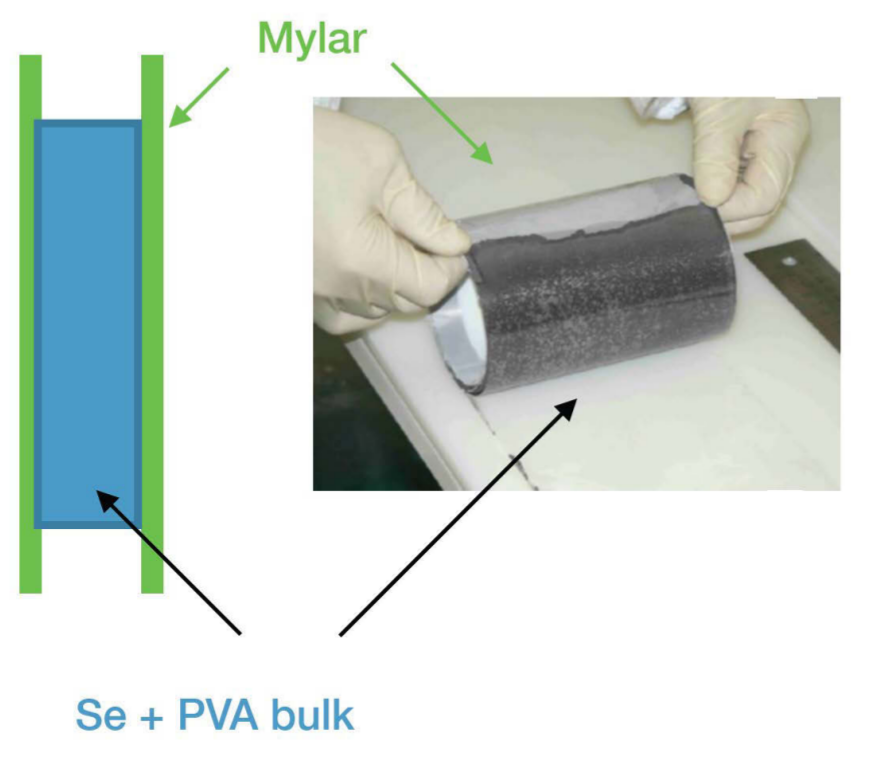
\includegraphics[scale=0.2]{pictures/Chap4/MylarDesign.png}
\caption{Schematic side view of the mylar design.}
\label{MylarDesign}
\end{figure}


\FloatBarrier


\subsubsection{TULLE}


\NI The TULLE design is a new design for the source foils in which the $^{\text{82}}$Se and the PVA paste is spread as uniform as possible over a thin layer of bobbinet tulle made of nylon6-6 providing a light and resistant mechanical support. A schematic view of the foil design is shown in Figure~\ref{TulleDesign}. The bobbinet tulle is constructed by warp and weft yarns in which the weft yarn is looped diagonally around the vertical warp yarn to form a hexagonal mesh which is regular and clearly defined.


\bigskip


\NI To minimise the contamination in $^{\text{208}}$Tl and $^{\text{214}}$Bi coming from the tulle, the lightest fabric available on the market has been chosen, corresponding to a weight of 0.7 mg/cm$^\text{2}$ and was not treated with resins nor paint after weaving. The tulle is ligher than the mylar backing film and gives the advantage of introducing a smaller contamination of $^{\text{208}}$Tl and $^{\text{214}}$Bi which will translate in lower background levels. Nevertheless, in this design, due to the lack of external protection the source foil is directly in contact with the gas in the tracker and is exposed to the risk of $^{\text{82}}$Se losses. In order to avoid this problem the amount of PVA can be increased to improve the foil strength. An increase of the amount of PVA will translate into a higher contamination and a higher thickness of the source foil. 


\begin{figure}[h!]
\centering
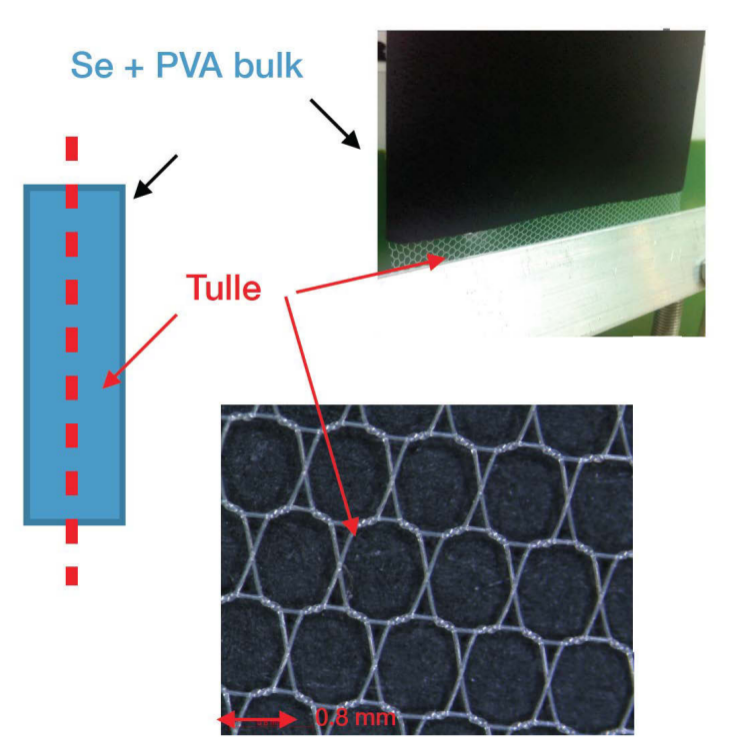
\includegraphics[scale=0.2]{pictures/Chap4/TulleDesign.png}
\caption{Schematic side view of the tulle design.}
\label{TulleDesign}
\end{figure}


\FloatBarrier


\subsection{Discussion}\label{sec:SourceFoilDesignDiscussion}


\NI The parameters used for the modelisation of the source foils for the different designs are summarized in Table~\ref{Tab:SummaryParametersSourceFoilDesign} and~\ref{Tab:ExpectedBkgSourceFoilDesign}. The case of the MYLAR foil, which is considered as an IDEAL foil with two external backing films, the parameters are shown separately for the bulk (b) and the film (f). The TULLE foil is modelled as an IDEAL foil with the nylon mesh uniformly distributed in the foil.


\bigskip


\NI As shown in Table~\ref{Tab:ExpectedBkgSourceFoilDesign}, from the radio-purity point of view, the TULLE design is very promising. Compared to the MYLAR design, even if more PVA is used, it allows to obtain a total activity in $^{\text{214}}$Bi and $^{\text{208}}$Tl which is respectively 18\% and 29\% lower. 



\begin{table}[h!]
\centering
\begin{tabular}{c|c|c|c|c|c|c}
\multirow{2}{*}{Design} & f$_\text{Se}$ & f$_\text{PVA}$ & f$_\text{Support}$ & a                  & $\rho$            & t \\
                        & [-]           & [-]            & [-]                & [mg/cm$^\text{2}$] & [g/cm$^\text{3}$] & [$\mu$m] \\[0.1cm]
\toprule
IDEAL & 0.95  & 0.05 & 0.00  & 52.5                             & 3.11 & 169 \\[0.1cm]
TULLE & 0.888 & 0.10 & 0.012 & 56.3                             & 2.98 & 189 \\[0.1cm]
MYLAR & 0.95  & 0.05 & -     & 52.5$_\text{b}$ + 3.2$_\text{f}$ & 3.11$_\text{b}$ + 1.4$_\text{f}$ & 169$_\text{b}$ + 24$_\text{f}$ \\[0.1cm]
\bottomrule
\end{tabular}
\caption{Summary of the foil parameters for the source foil designs under consideration. The MYLAR design is considered as IDEAL with two external backing films. The parameters in this case are then shown separately for the bulk (b) and the film (f).}
\label{Tab:SummaryParametersSourceFoilDesign}
\end{table}



\begin{table}[h!]
\centering
\begin{tabular}{c|c|c|c|c|c}
\multirow{2}{*}{Design} & f$_\text{Se}$/f$_\text{Se}$ & f$_\text{PVA}$/f$_\text{Se}$ & f$_\text{Support}$/f$_\text{Se}$ & A ($^{\text{214}}$Bi) & A ($^{\text{214}}$Bi)  \\
& [-]   & [-]   & [-]   & [$\mu$Bq/kg] & [$\mu$Bq/kg] \\[0.1cm]
\toprule
IDEAL & 1 & 0.053 & 0.000 & 62.0                               & 3.4   \\[0.1cm]
TULLE & 1 & 0.113 & 0.014 & 142.5                              & 13.5  \\[0.1cm]
MYLAR & 1 & 0.053 & 0.068 & 62.0$_\text{b}$ + 111.6$_\text{f}$ & 3.4$_\text{b}$ + 15.6$_\text{f}$  \\[0.1cm]
\bottomrule
\end{tabular}
\caption{Expected $^{\text{208}}$Tl and $^{\text{214}}$Bi activities computed from~Equation~\ref{eq:ActivityComponent}. The values do not include the activity of the $^{\text{82}}$Se which is not known at this stage.}
\label{Tab:ExpectedBkgSourceFoilDesign}
\end{table}


\FloatBarrier


\section{Monte-Carlo simulations}\label{sec:MCsimulations}


\NI The study performed in this work is based on the event simulation performed through the software developed by the collaboration The propagation of the particles through the detector is performed by a GEANT4 based module which simulates all relevant processes, such as multiple scattering, ionisation, Compton scattering, Bremsstrahlung. The detector response is then obtained by smearing the true information provided by GEANT4 with respect to the calorimeter and the tracker resolution. Dedicated reconstruction and selection modules allow selecting events in a specific channel for dedicated analysis.


\bigskip


%\NI This work is not meant to document and validate the Falaise-legacy chain, a complete validation of the framework should be found elsewhere. The description available in the following focuses only on the parts relevant for this work. Moreover, the Falaise-legacy is likely to be abandoned in favour of a new version of the framework which is currently under validation. The new software should be used in the future to cross-check the MC production used for this work.


\subsection{Source foils modelisation}


\NI The modelisation of the source foils is realized through rectangular boxes made of $^{\text{82}}$Se, PVA, nylon or mylar depending on from the design under consideration. The composition of the different designs introduced in Section~\ref{sec:designUnderConsideration} are used as well as the parameters summarised in Table~\ref{Tab:SummaryParametersSourceFoilDesign}. The implementation of the material composition is performed by defining the fraction mass for each element, mainly $^{\text{82}}$Se, $^{\text{Nat}}$Se, O, C and N which is found in the nylon mesh.


\subsection{Event generation}


\NI The generation of the events is performed uniformly from the source foil. They are generated for the 0$\nu\beta\beta$, 2$\nu\beta\beta$ and the internal background coming from contamination in $^{\text{208}}$Tl and $^{\text{214}}$Bi. For the MYLAR design, to take into account the contamination coming from the backing film, events of $^{\text{208}}$Tl and $^{\text{214}}$Bi are also generated in the mylar film. Table~\ref{Tab:GeneratedEventSource} shows the statistics generated for each event type. 


\begin{table}[h!]
\centering
\begin{tabular}{c|c|c|c|c}
Design & 0$\nu\beta\beta$ & 2$\nu\beta\beta$ & $^{\text{208}}$Tl & $^{\text{214}}$Bi  \\[0.1cm]
\toprule
IDEAL & 10$^{\text{6}}$ & 10$^{\text{7}}$ & 10$^{\text{7}}$ & 10$^{\text{7}}$  \\[0.02cm]
TULLE & 10$^{\text{6}}$ & 10$^{\text{7}}$ & 10$^{\text{7}}$ & 10$^{\text{7}}$  \\[0.02cm]
MYLAR &                 &                 &                 &                  \\[0.02cm]
(bulk)& 10$^{\text{6}}$ & 10$^{\text{7}}$ & 10$^{\text{7}}$ & 10$^{\text{7}}$  \\[0.02cm]
(film)&                 &                 & 10$^{\text{7}}$ & 10$^{\text{7}}$  \\[0.02cm]
\bottomrule
\end{tabular}
\caption{Generated statistics for each event type and source foil design.}
\label{Tab:GeneratedEventSource}
\end{table}


\NI Since the event generation has been performed with many different configurations of the source foil, the statistics has been optimised to contain the event production within reasonable processing time (24 hours).  This current production allows to keep the statistical uncertainty on the number of events selected in the relevant energy region within 0.2\% for the 0$\nu\beta\beta$ and the 2$\nu\beta\beta$ events and within 5\% for the 208 Tl and 214 Bi events which is already a factor 2 lower than the systematic uncertainties observed for the internal background in NEMO-3 (10\%). As these systematics are expected to be similar in SuperNEMO, we consider that the statistics of the MC samples is enough in this context.


\subsection{Energy distribution}\label{sec:EventsEnergyDistribution}


\NI The reconstruction of the events and the selection of the 2e channel is then performed. Only the events having two negative tracks hitting two calorimeter blocks with a total energy deposition E$_{\beta\beta}$ > 2 MeV are selected. The energy distributions for the signal and the backgrounds are shown in Figure~\ref{Distribution2eSelection}. These p.d.f will be used therafter to compare among different designs of the source foil. The IDEAL design is shown in black, the TULLE design in red and the MYLAR design in blue. From these distributions it can be seen that the shape of the energy distribution do not depend heavily on the considered design even if a small overall decrease of the event selection efficiency is observed for the TULLE and MYLAR design compared to the IDEAL case. This decrease is more important for the 0$\nu\beta\beta$ and 2$\nu\beta\beta$ while it is not significant for the $^{\text{208}}$Tl and $^{\text{214}}$Bi. The effect is due to the increased thickness of the source foil in the TULLE and the MYLAR designs compared to the IDEAL case, which slightly shifts the p.d.f to the lower energies due to an increased energy loss in the foil. The selection efficiency for the signal and the background obtained in the [2000; 3200] keV energy window are shown in Table~\ref{Tab:EventSelectionEfficiency}.


\begin{figure}[h!]
\centering
%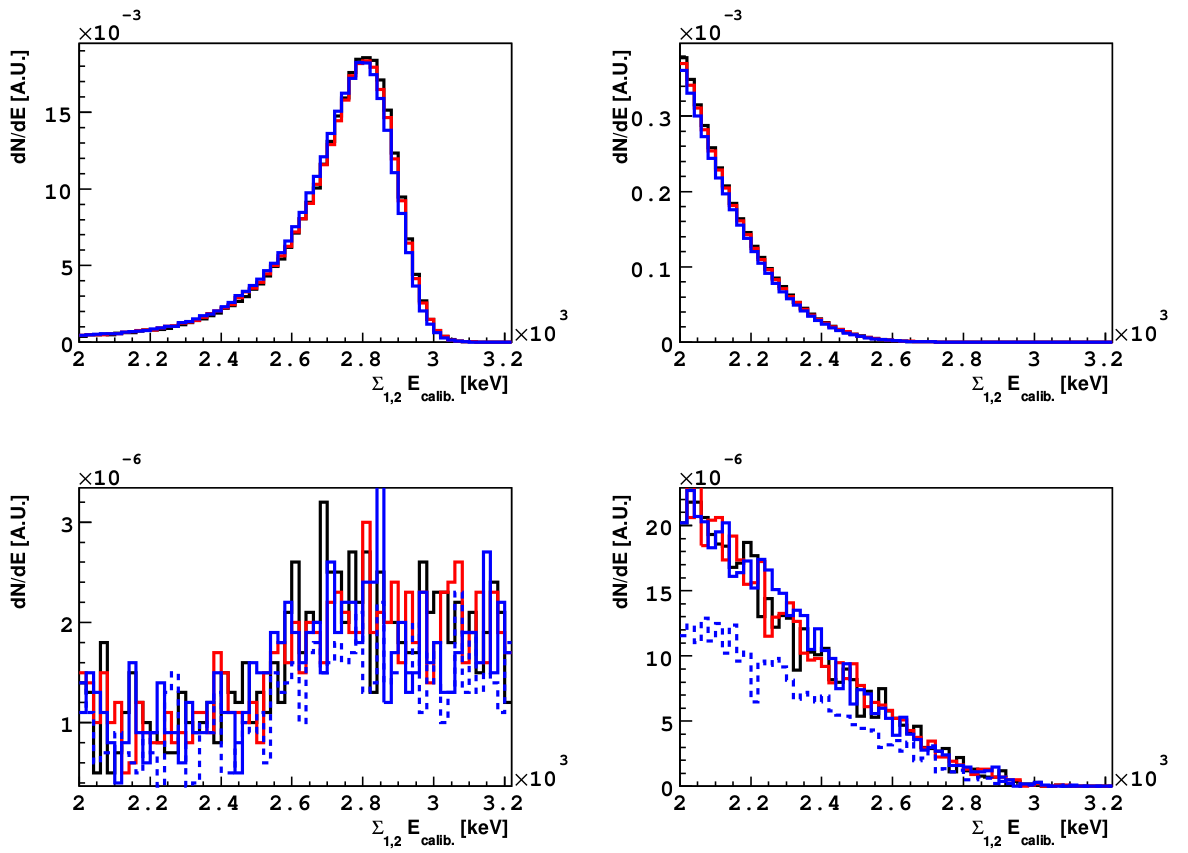
\includegraphics[scale=0.24]{pictures/Chap4/Distribution2eSelection.png}
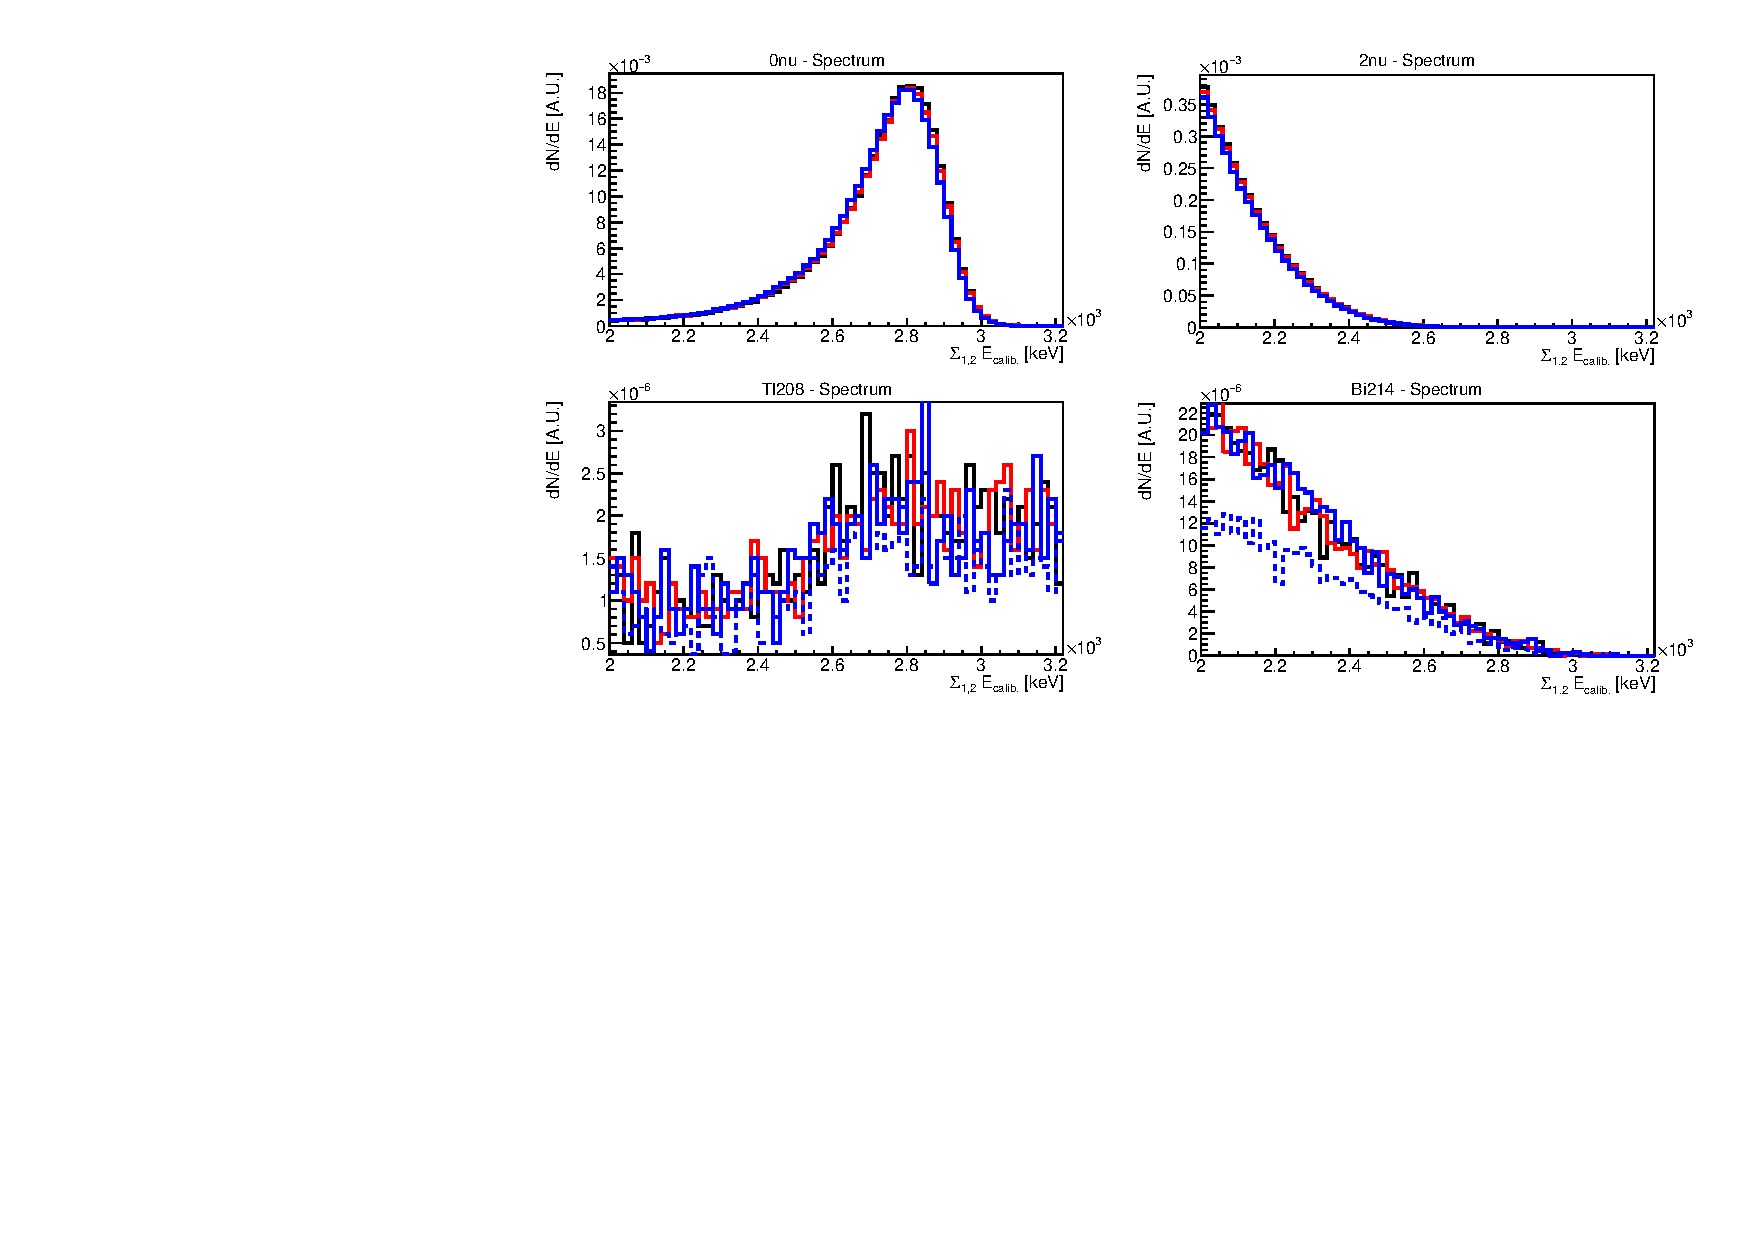
\includegraphics[scale=0.65]{pictures/Chap4/Distribution2eSelection_v2.pdf}
\caption{Comparaison of the 2e energy distribution for signal and background channels for different source foil designs. Black IDEAL. Red : TULLE. Blue : MYLAR. Top left : 0$\nu\beta\beta$, top right : 2$\nu\beta\beta$, bottom left : $^{\text{208}}$Tl, bottom right : $^{\text{214}}$Bi. The dashed blue histogram in the bottom plots represent the expected energy for events generated in the mylar backing film.}
\label{Distribution2eSelection}
\end{figure}


\begin{table}[h!]
\centering
\begin{tabular}{c|c|c|c|c}
\toprule
\multirow{2}{*}{Design} & $\epsilon_{\text{0}\nu}$ & $\epsilon_{\text{2}\nu}$ & $\epsilon_{\text{Tl}}$ & $\epsilon_{\text{Bi}}$  \\
& [\%]   & $\times$ 10$^{-\text{2}}$ [\%] & $\times$ 10$^{-\text{2}}$ [\%] & $\times$ 10$^{-\text{2}}$ [\%] \\[0.1cm]
\hline
IDEAL & 29.01 $\pm$ 0.05 & 33.64 $\pm$ 0.04 & 0.99 $\pm$ 0.03 & 4.3 $\pm$ 0.1 \\[0.05cm]
\hline
TULLE & 28.84 $\pm$ 0.04 & 33.05 $\pm$ 0.04 & 0.95 $\pm$ 0.03 & 4.4 $\pm$ 0.1 \\[0.05cm]
\hline
MYLAR & & & & \\[0.1cm]
(bulk)& 28.86 $\pm$ 0.04 & 31.75 $\pm$ 0.04 & 0.92 $\pm$ 0.03 & 4.5 $\pm$ 0.1 \\[0.05cm]
(film)& & & 0.73 $\pm$ 0.03 & 2.7 $\pm$ 0.1 \\ 
\bottomrule
\end{tabular}
\caption{Event selection efficiency in the 2e channel in [2000; 3200] keV.}
\label{Tab:EventSelectionEfficiency}
\end{table}


\FloatBarrier


\section{Sensitivity study}\label{sec:SensStudy}


%\NI The study of the sensitivity of an experiment looking for a new phenomena, allows to estimate its physics case and compare among different competing experiments. During the designing phase, it is also useful to study the sensitivity with respect to different detector configurations in order to find the optimal design.


\NI In order to define the sensitivity to a phenomenon not yet observed, we assume the experiment does not observe any signal. In this worse case scenario, we study which portion of the allowed parameter phase space the experiment can exclude. The p.d.fs obtained in the previous chapter with the IDEAL design are used in the following as example of sensitivity computation. Here the backgrounds are normalised to 2~$\mu$Bq/kg and 10~$\mu$Bq/kg for the $^{\text{208}}$Tl and the $^{\text{214}}$Bi internal background respectively (i.e. the target radio-purity level of SuperNEMO). The 2$\nu\beta\beta$ background is normalised to 9~$\times$~10$^{\text{19}}$~y as measured in NEMO-3~\cite{NEMO3-BKG}. This configuration is referred in the text as IDEAL$^{\star}$.


\subsection{R.O.I method}\label{sec:ROImethod}


\NI As defined in Section~\ref{sec:ExperimentalSearch0nu}, the sensitivity on the 0$\nu\beta\beta$ decay half-life is given by~:


\begin{equation}\label{eq:limitHalfLife}
\text{T}_{\text{1/2}}^{\text{0}\nu} > \frac{\text{N}_\text{A}~\text{ln2}}{\text{W}} \times \frac{\epsilon \times \text{M} \times \text{T}}{\mathcal{S}(\text{b})}
\end{equation}


\NI where N$_\text{A}$ is the Avogadro number, W the atomic mass of the $\beta\beta$ isotope under study, $\epsilon$ is the signal selection efficiency and M $\times$ T the total experimental exposure. The $\mathcal{S}$(b) term represents the average upper limit on the number of signal events that would be obtained by an ensemble of identical replicas of such experiments, each one with the same mean expected background and no true signal. The Feldman \& Cousins unified approach for the definition of the confidence level is adopted. This method optimises the region of interest (R.O.I.) with respect to the sensitivity to the T$_{\text{1/2}}^{\text{0}\nu}$. This optimisation is achieved by maximising the $\epsilon$/S(b) ratio for a given exposure M~$\times$~T.


\subsection{Selection efficiency}


\NI The signal and the background selection efficiencies in the 2e channel are obtained by integrating the respective p.d.f. in the R.O.I. defined by the energy window (E$_{\text{low}}$, E$_{\text{up}}$) : 


\begin{equation}\label{eq:CompuationEfficiency}
\epsilon_\text{i} (\text{E}_{\text{low}};\text{E}_{\text{up}}) = \frac{1}{\text{N}} \int_{\text{E}_{\text{low}}}^{\text{E}_{\text{up}}} \frac{\text{dN}}{\text{dE}} \text{dE}
\end{equation}


\bigskip


\NI Figure~\ref{SelectionEfficiency} shows the value of efficiency for the 0$\nu\beta\beta$ signal (red) and background (2$\nu\beta\beta$ in blue, 214 Bi in yellow and 208 Tl in green) when the upper edge of the R.O.I. is kept fixed at 4500~keV while the lower edge is moved from 2000~keV up to 3500~keV. These efficiencies are then used to estimate the expected background level for a given exposure M~$\times$~T following~:


\begin{equation}\label{eq:Nbkg2nu}
\text{N}_{\text{2}\nu} = \frac{\text{N}_\text{A}~\text{ln2}}{\text{W}} \times \frac{\epsilon_{\text{2}\nu} \times \text{M} \times \text{T}}{\text{T}_{\text{1/2}}^{\text{2}\nu}}
\end{equation}


\begin{equation}\label{eq:NbkgBi214}
\text{N} (^{\text{214}}\text{Bi}) = \text{A} (^{\text{214}}\text{Bi}) \times \epsilon (^{\text{214}}\text{Bi}) \times \text{M} \times \text{T} 
\end{equation}


\begin{equation}\label{eq:NbkgTl208}
\text{N} (^{\text{208}}\text{Tl}) = \text{A} (^{\text{208}}\text{Tl}) \times \epsilon (^{\text{208}}\text{Tl}) \times \text{M} \times \text{T} 
\end{equation}


\NI Where T$_{\text{1/2}}^{\text{2}\nu}$ is the measured half-life for the 2$\nu\beta\beta$ decay, and A($^{\text{214}}$Bi) and A($^{\text{208}}$Tl) are the expected activity level of $^{\text{214}}$Bi and $^{\text{208}}$Tl contamination of the foil source. The expected number of background events as a function of the low energy edge of the R.O.I is provided by the renormalisation of the histogram given in Figure~\ref{SelectionEfficiency} through the Equations~\ref{eq:Nbkg2nu},~\ref{eq:NbkgBi214} and~\ref{eq:NbkgTl208} and is shown in Figure~\ref{ExpectedNumberofEvent}.


\bigskip


\NI Instead of fixing the value of E$_\text{\text{up}}$ when computing the integral of Equation~\ref{eq:CompuationEfficiency}, both edges of the R.O.I can be changed to obtain a 2D scan of the selection efficiencies. As proceeded before, the same renormalisation through Equations~\ref{eq:Nbkg2nu},~\ref{eq:NbkgBi214} and~\ref{eq:NbkgTl208} provides the 2D scan of the expected number of background events w.r.t. the edges of the R.O.I. as shown in Figure~\ref{BkgCount2D}.



\begin{figure}[h!]
\centering
%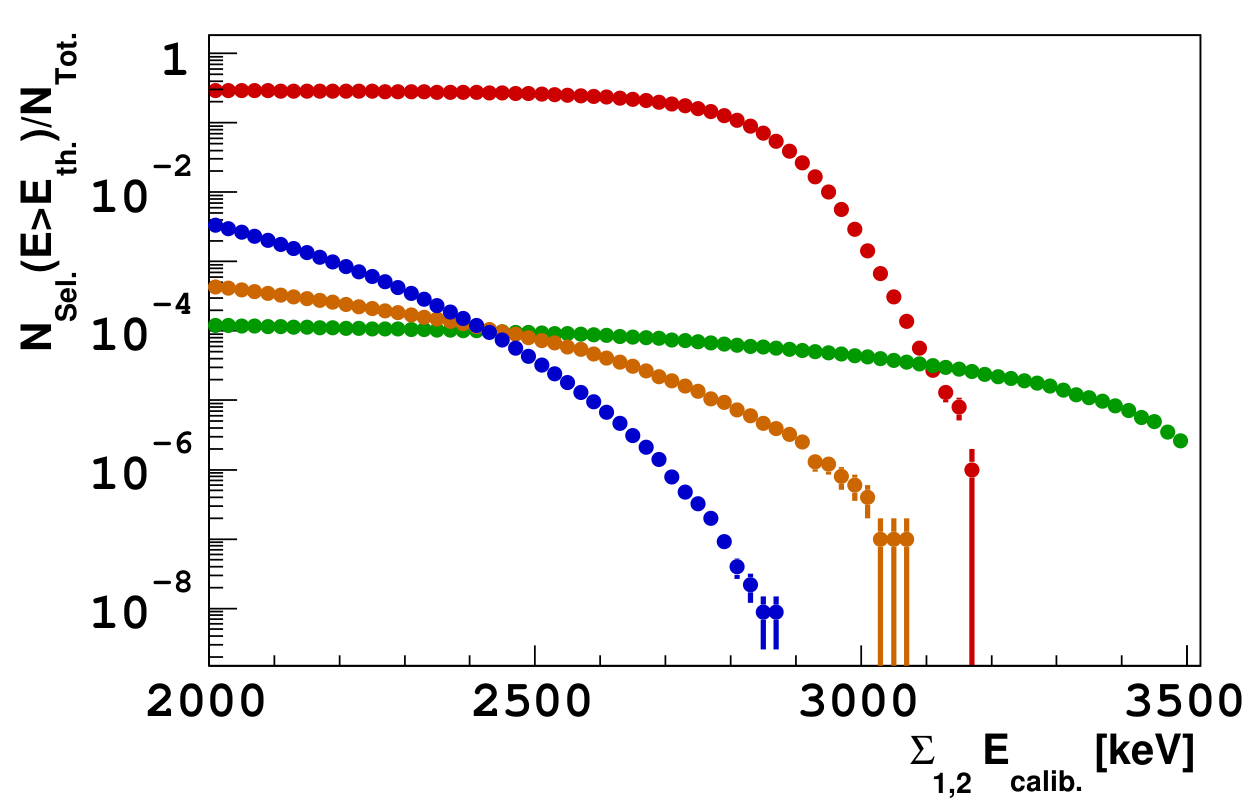
\includegraphics[scale=0.25]{pictures/Chap4/SelectionEfficiency.png}
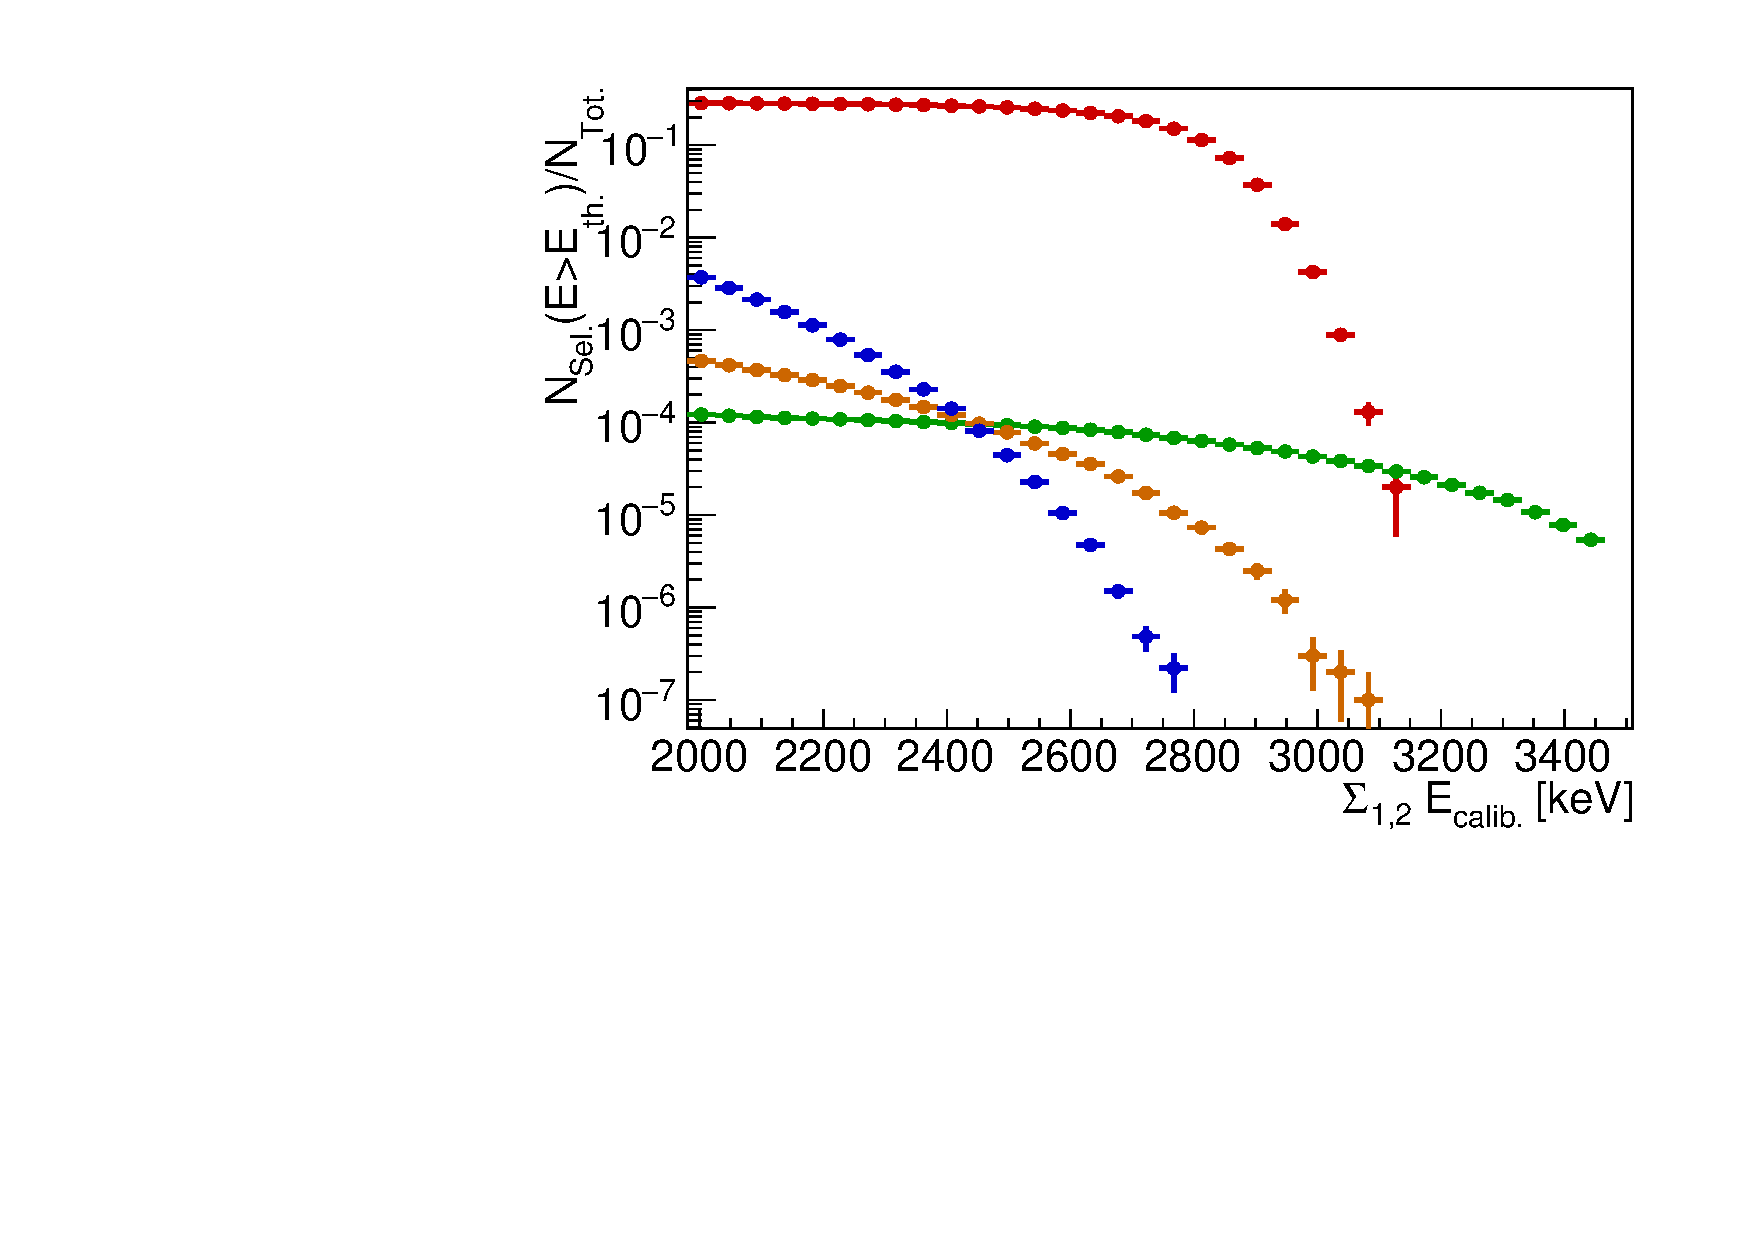
\includegraphics[scale=0.6]{pictures/Chap4/EffExample.pdf}
\caption{Selection efficiency for the 0$\nu\beta\beta$ signal (red) and the different backgrounds (2$\nu\beta\beta$ in blue, $^{\text{214}}$Bi in yellow and $^{\text{208}}$Tl in green). The upper edge of the R.O.I is kept fixed at 4500~keV while the lower edge is moved from 2000~keV up to 3500~keV.}
\label{SelectionEfficiency}
\end{figure}


\begin{figure}[h!]
\centering
%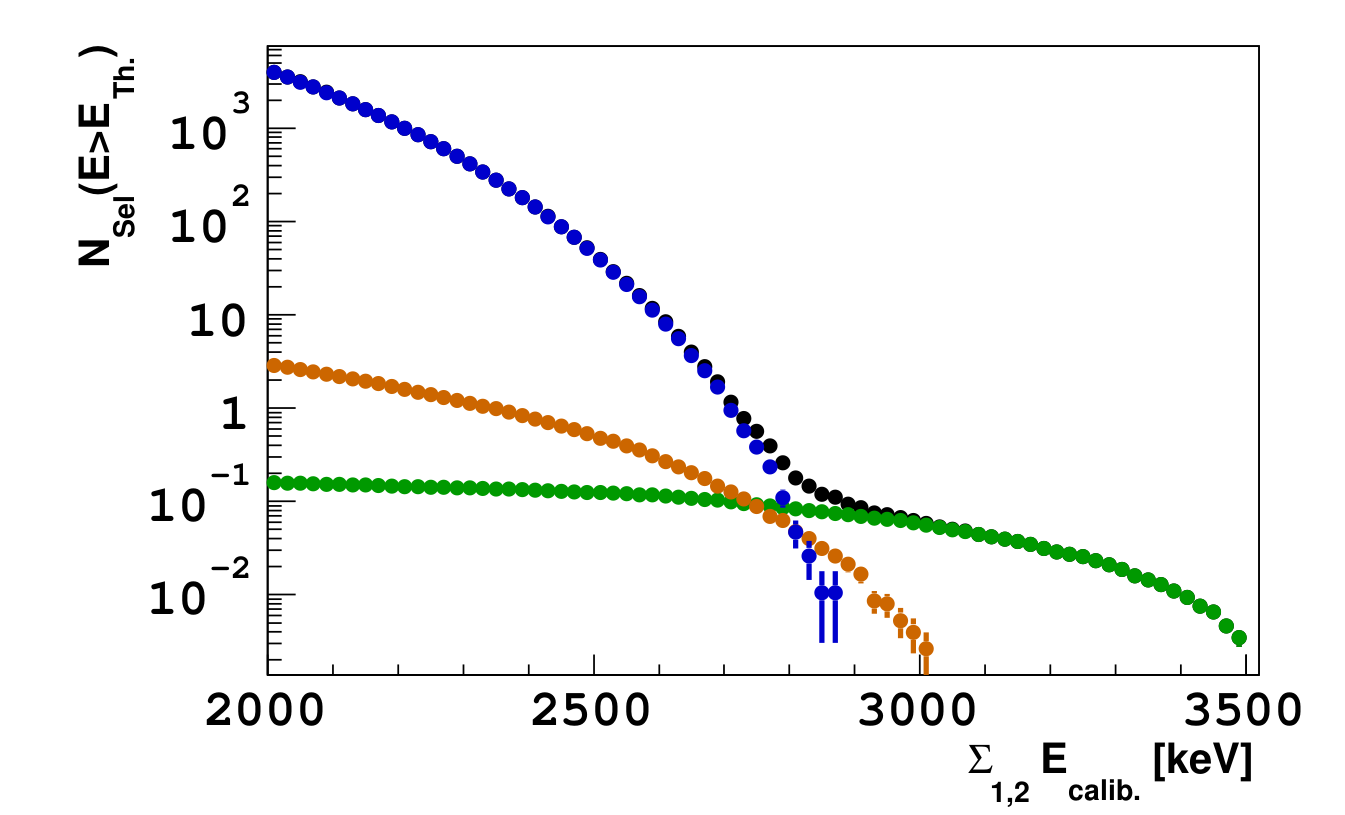
\includegraphics[scale=0.25]{pictures/Chap4/ExpectedNumberofEvent.png}
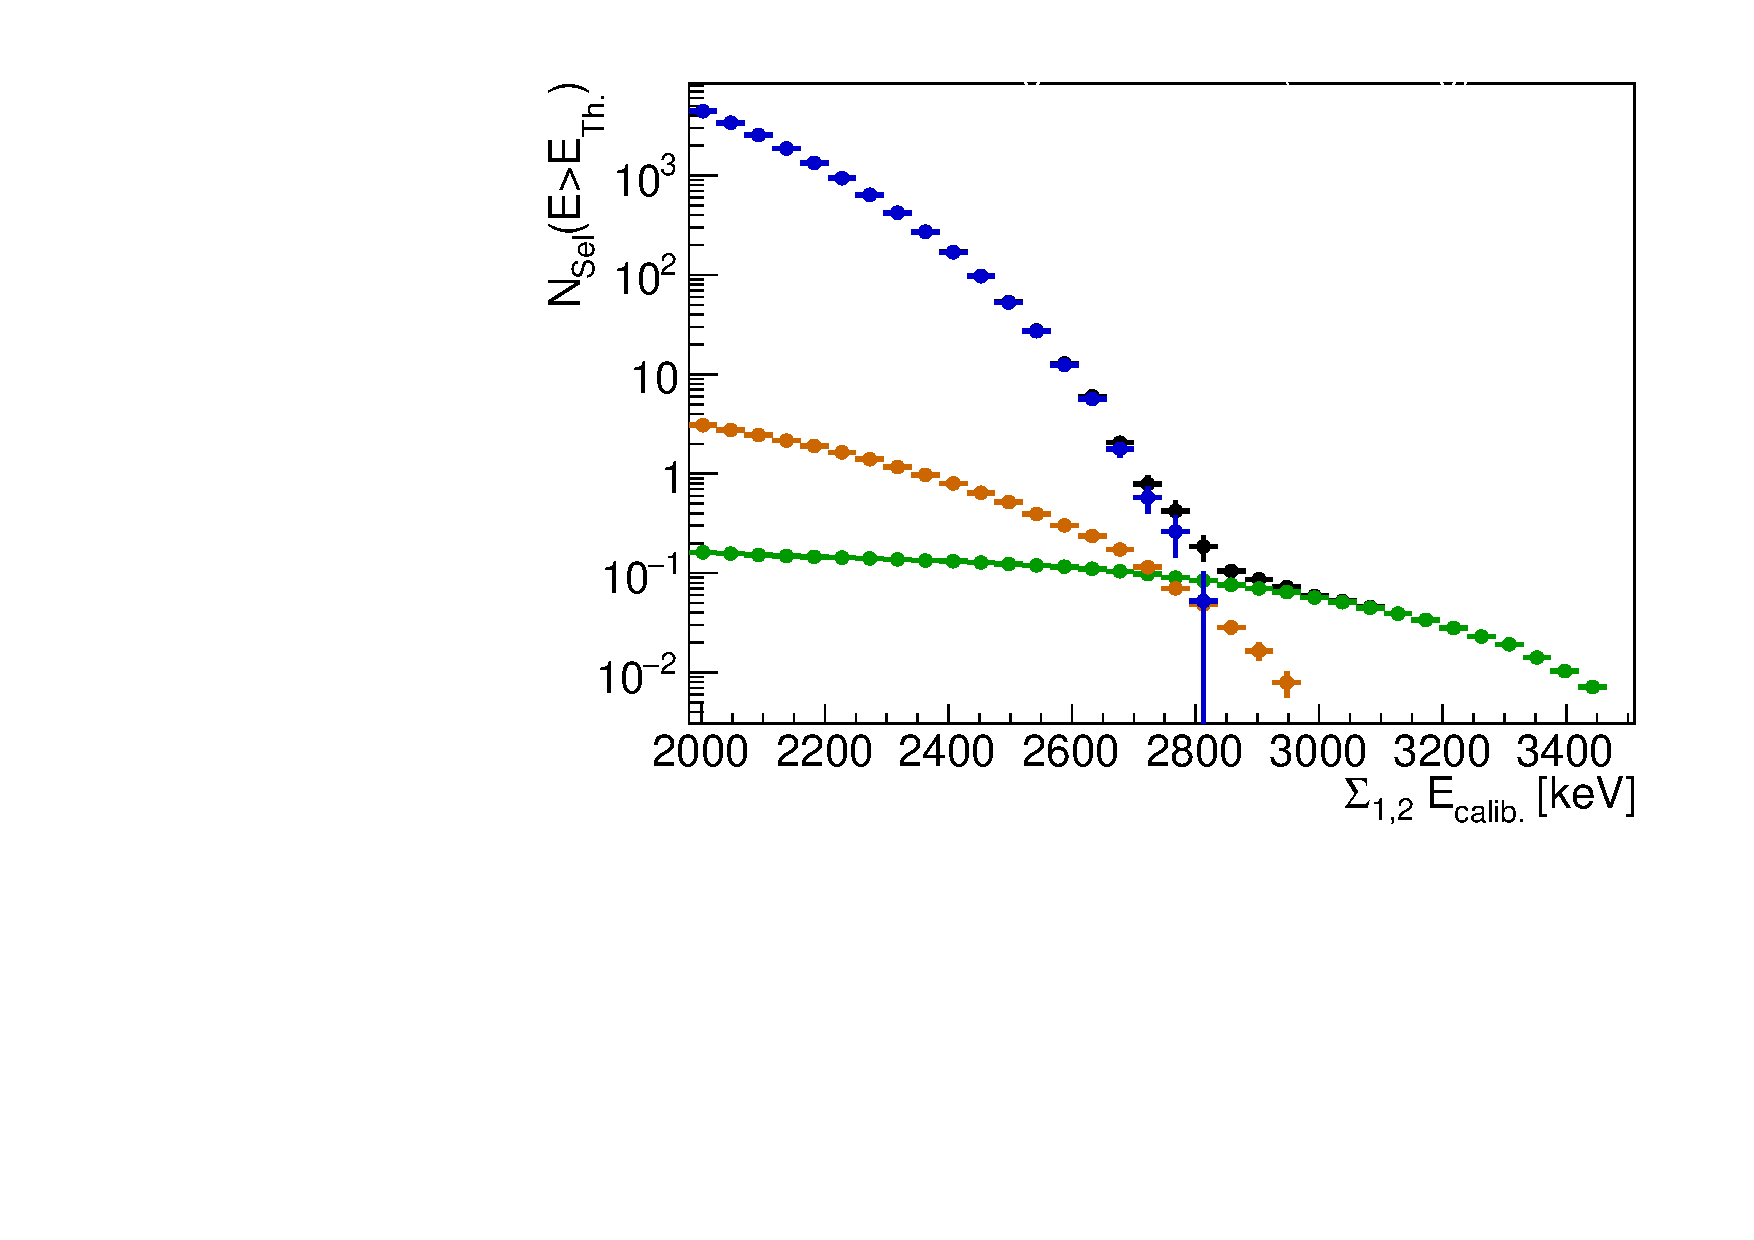
\includegraphics[scale=0.6]{pictures/Chap4/BkgExample.pdf}

\caption{Expected number of background events (2$\nu\beta\beta$ in blue, $^{\text{214}}$Bi in yellow and $^{\text{208}}$Tl in green) as a function of the low energy edge of the R.O.I. The black points show the sum of all background contributions.}
\label{ExpectedNumberofEvent}
\end{figure}


\begin{figure}[h!]
\centering
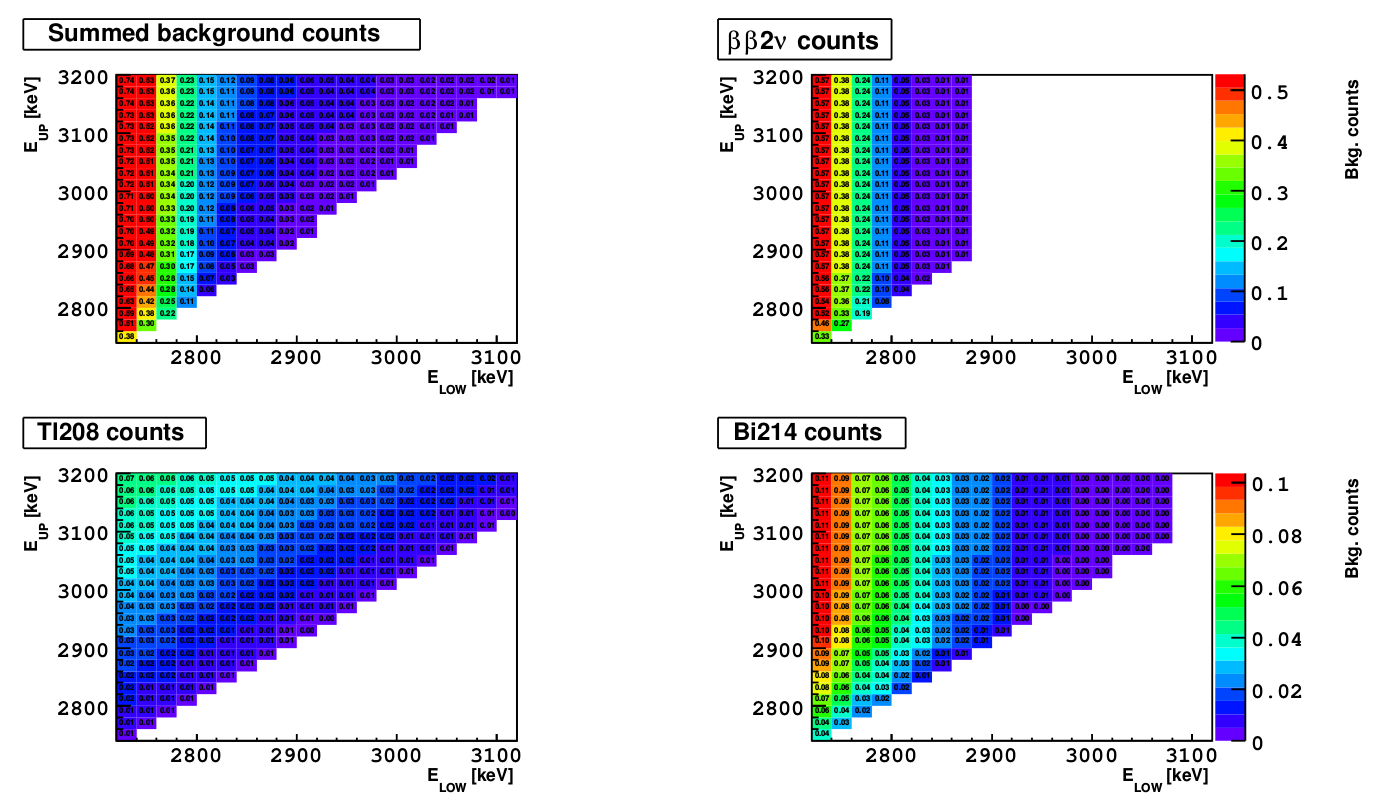
\includegraphics[scale=0.4,  angle =90]{pictures/Chap4/BkgCount2D}
\caption{Expected background counts as a function of the edges of the R.O.I..}
\label{BkgCount2D}
\end{figure}


\FloatBarrier


\subsection{The Feldman \& Cousins 90\% C.L.}
 

\NI The $\mathcal{S}$(b) term of Equation~\ref{eq:limitHalfLife} is defined following the Feldman \& Cousins prescription for the definition of confidence interval of small signal~\cite{FeldmanCousins}. Defining U(n$|$b) as the function yielding the (unified approach) upper limit (at the desired C.L.) for a given observation n and a mean predicted background level b. Given that the variable n follows a Poisson p.d.f., P(n$|$b) = P(n; b), then $\mathcal{S}$(b) is given by : 


\begin{equation}
\mathcal{S}(\text{b}) = \text{E}[\mathcal{U}(\text{n}|\text{b})] = \sum_{\text{n}=0}^{\infty} \mathcal{P} (\text{n};\text{b}) \times \mathcal{U}(\text{n}|\text{b})
\end{equation}


\NI The sensitivity $\mathcal{S}$(b) of an experiment expecting b events of background and no true signal is obtained by averaging the upper limits obtained using the unified approach U(n$|$b) with the likelihood of the individual observations P(n$|$b). Figure~\ref{FeldmanAndCousin} shows the 90\% C.L. curve for a background level spanning in [0; 40] c.t.s. Note that in the large background approximation, the sensitivity curve as a function of b follows the expected classical limit obtained through the Neyman construction of the confidence belt, with a~=~1.64~(1.96) at 90\%~(95\%) C.L. : $\mathcal{S}(\text{b}) \propto \text{a} \times \sqrt{\text{b}}, ~\text{for}~\text{large}~\text{b}$. 	


\begin{figure}[h!]
\centering
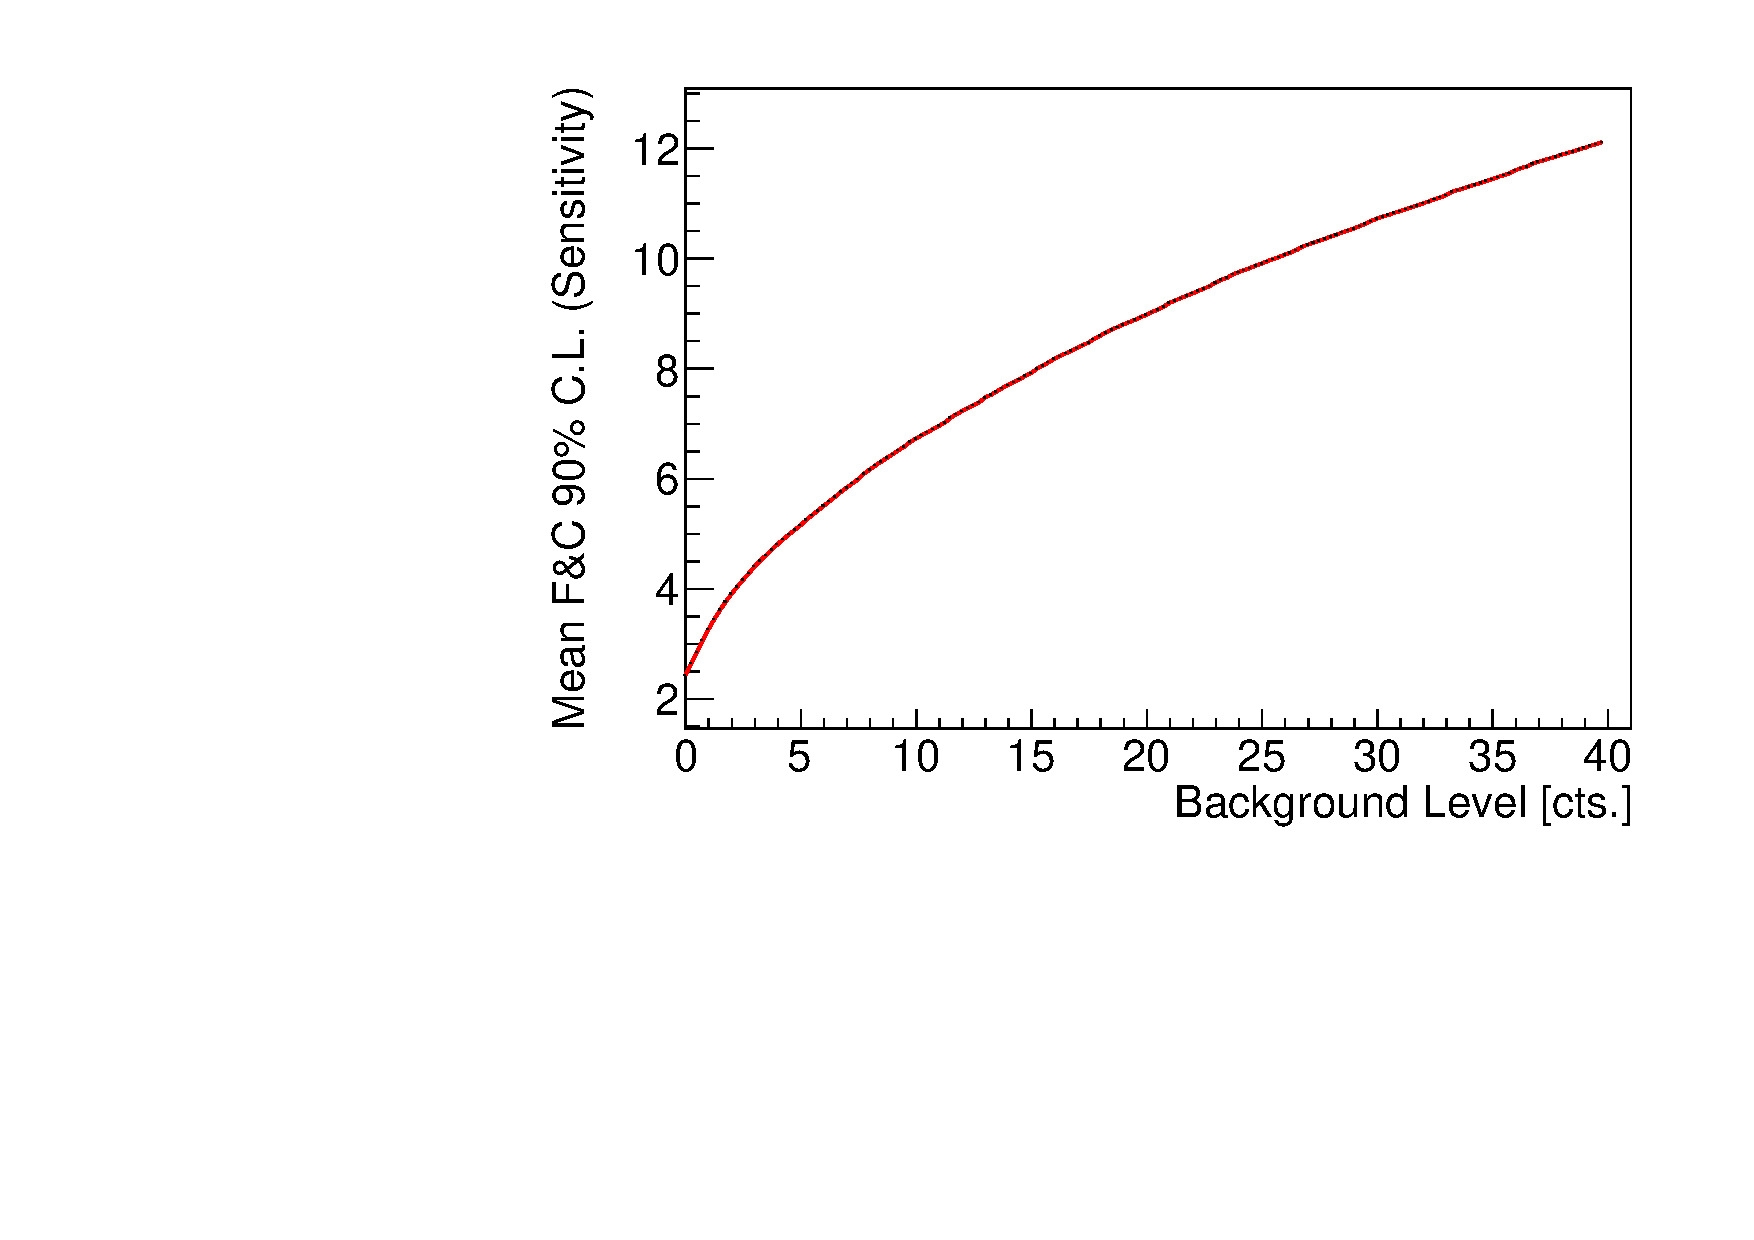
\includegraphics[scale=0.45]{pictures/Chap4/FeldmanCousin.pdf}
\caption{The 90\% C.L. sensitivity curve as a function of the number of background events.}
\label{FeldmanAndCousin}
\end{figure}


\FloatBarrier


\subsection{1d vs 2d R.O.I. optimisation}


\NI By using Equation~\ref{eq:limitHalfLife}, the sensitivity is computed as a function of the R.O.I for a given experimental exposure. Figure~\ref{Sens0nu1D} shows the 1d sensitivity scan as a function of the low energy edge of the R.O.I. for an exposure of 21 kg$\times$y.  The best sensitivity is found to be 6.1$\times$10$^{\text{24}}$~y in the energy window of [2720; 3200] keV. The expected total background contamination in the region is of 0.74~$\pm$~0.06 cts. The same strategy is applied for the 2d optimisation of the R.O.I, except both edges simultaneously vary to optimise the R.O.I.. The best sensitivity of 6.12$\times$10$^{\text{24}}$~y is found in [2720; 3060]~keV, with an expected total background contamination of 0.72~$\pm$~0.06~cts. No major reduction of the background is observed, the results are found to be compatible within the statistical uncertainties. 


\begin{figure}[h!]
\centering
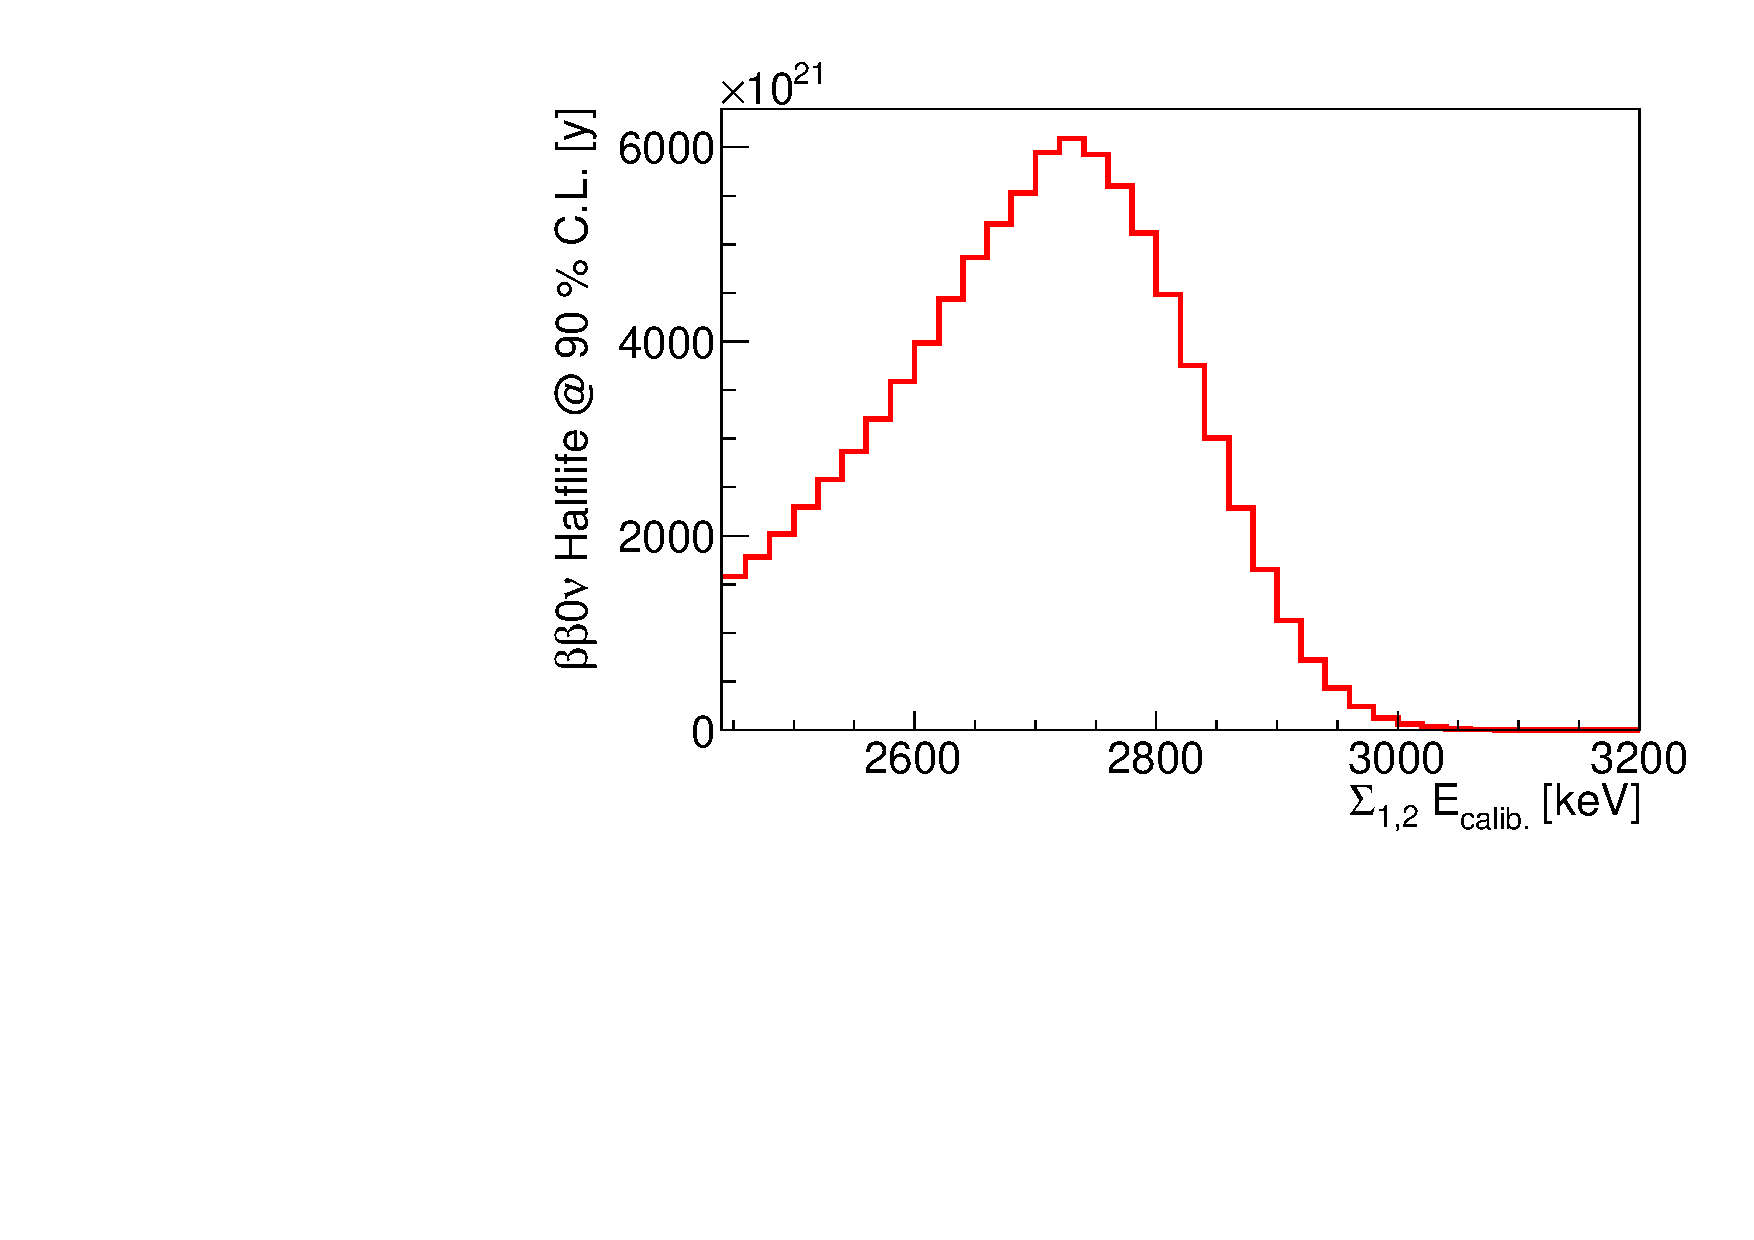
\includegraphics[scale=0.45]{pictures/Chap4/Sens1D.pdf}
\caption{The 1d sensitivity scan as a function of the low energy edge of the R.O.I.. The high energy edge is kept fixed at 3200 keV. The best sensitivity of 6.1$\times$10$^{\text{24}}$~y is found in [2720; 3200] keV after 21 kg$\times$y exposure, with an
expected total background contamination of 0.74 $\pm$ 0.06 cts.}
\label{Sens0nu1D}
\end{figure}


\begin{figure}[h!]
\centering
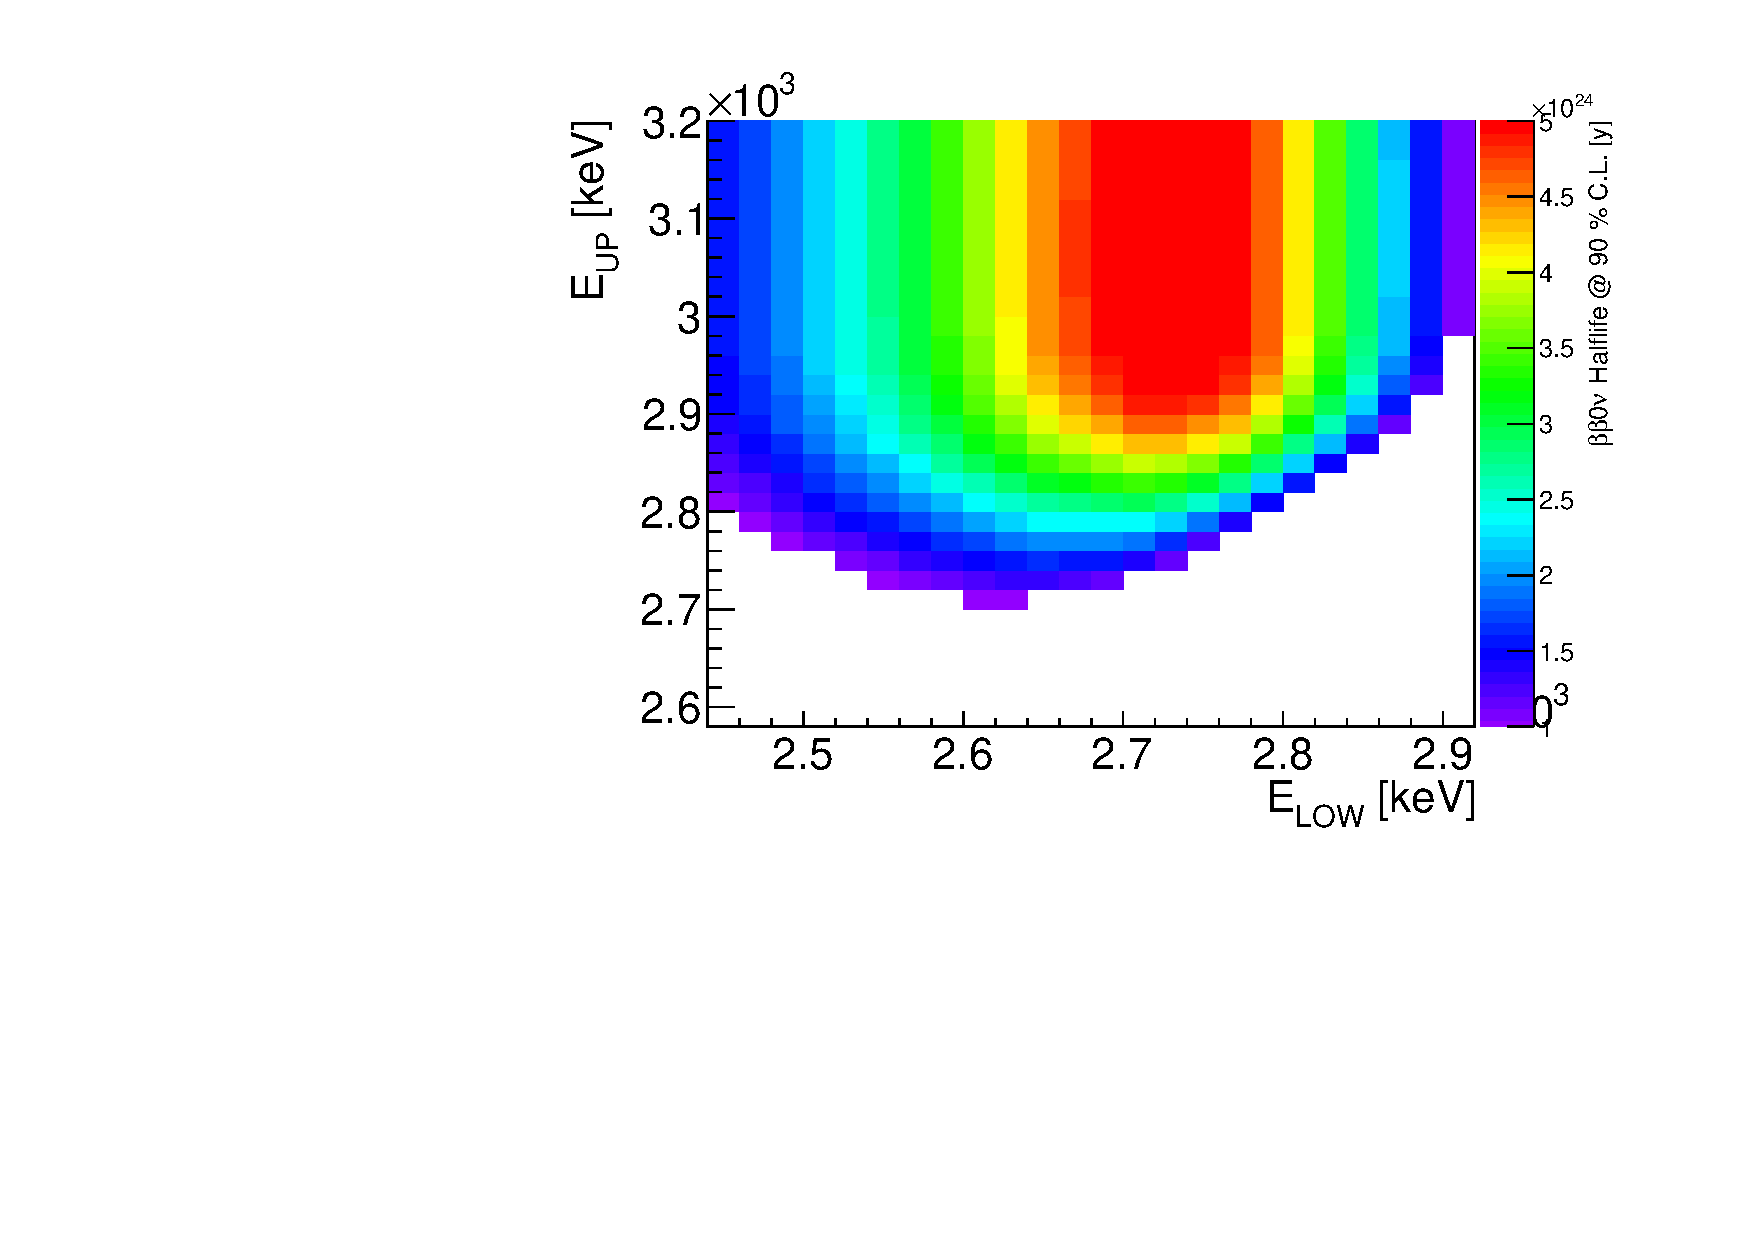
\includegraphics[scale=0.45]{pictures/Chap4/sens2D.pdf}
\label{Sens0nu2D.png}
\caption{The 2d sensitivity scan as a function of the energy edges of the R.O.I.. The best sensitivity of 6.12$\times$10$^{\text{24}}$~y is found in [2720; 3060] keV after 21 kg$\times$y exposure, with an expected total background contamination of 0.72 $\pm$ 0.06 cts.}
\end{figure}


\FloatBarrier


\subsection{Validation of the background level}


\NI The NEMO-3 results on the $^{\text{100}}$Mo~\cite{NEMO3:Mo100} can be used to crosscheck the background level obtained in Section~\ref{sec:ROImethod}. The background measured in NEMO-3 for $^{\text{214}}$Bi and $^{\text{208}}$Tl can be incorporated in Equations~\ref{eq:Nbkg2nu},~\ref{eq:NbkgBi214} and~\ref{eq:NbkgTl208} which are normalised to the exposure of the SuperNEMO demonstrator. Table~\ref{tab:ExtrapolationBackground} shows the internal $^{\text{208}}$Tl and $^{\text{214}}$Bi activities measured in NEMO-3, the measured background level in [2.8; 3.2] MeV and its extrapolation to the activities and exposure expected for the SuperNEMO demonstrator. The expected background levels extracted from Figure~\ref{BkgCount2D}, considering the same R.O.I. as NEMO-3, is presented in the last column.


\bigskip


\NI A difference of 33\% and 42\% is observed for the $^{\text{208}}$Tl and the $^{\text{214}}$Bi respectively. Note that a direct comparison could not be applied since NEMO-3 and SuperNEMO are not the same detector. SuperNEMO has a better energy resolution (8\% at 1 MeV w.r.t. the 14\% of NEMO-3) and a higher detection efficiency due to an optimised design of the tracker and the calorimeter. NEMO-3 has a 0$\nu\beta\beta$ detection efficiency of 4.7\% in [2.8; 3.2] MeV, for SuperNEMO this value is 11\%, as obtained from the simulation performed in this work. Neglecting the different energy resolutions ($^{\text{208}}$Tl and the $^{\text{214}}$Bi spectra are rather flat in the R.O.I.) the values of Table~\ref{tab:ExtrapolationBackground} agree within 20\% when considering that the 0$\nu\beta\beta$ selection efficiency of SuperNEMO is $\times$ 2.3 higher than NEMO-3.


\begin{table}[h!]
\centering
\begin{tabular}{c|c|c|c|c|c}
\toprule
 & \multicolumn{2}{c|}{NEMO-3}                    & \multicolumn{2}{c|}{Extrapolation} & Expectation         \\ [0.1cm]
 & \multicolumn{2}{c|}{$^{\text{100}}$Mo results} & \multicolumn{2}{c|}{to SuperNEMO}  & (simulation)        \\ [0.1cm]
\hline
 & Activities   & Events                          & Activities   & Events              & Events              \\ [0.1cm]
 & [$\mu$Bq/kg] & in 22 kg $\times$ y             & [$\mu$Bq/kg] & in 21 kg $\times$ y & in 21 kg $\times$ y \\ [0.1cm]
\hline
$^{\text{208}}$Tl & 128 $\pm$ 3 & 2.39 $\pm$ 0.22 & < 2 & 0.036 $\pm$ 0.004 & 0.054 $\pm$ 0.003 \\ [0.1cm]
$^{\text{214}}$Bi & 380 $\pm$ 40& 0.92 $\pm$ 0.13 & < 10& 0.028 $\pm$ 0.004 & 0.048 $\pm$ 0.006 \\ [0.1cm]
\bottomrule
\end{tabular}
\caption{The internal $^{\text{208}}$Tl and $^{\text{214}}$Bi activities measured in NEMO-3, the measured background level in [2.8; 3.2] MeV and its extrapolation to the activities and exposure expected for the SuperNEMO demonstrator. The last column shows the expected background level obtained from the calculation of sec. 4.1, considering the same R.O.I. as NEMO-3.}
\label{tab:ExtrapolationBackground}
\end{table}


\FloatBarrier


%\subsection{Validation of the sensitivity calculation}


%\NI The sensitivity value obtained with the extended likelihood method in sec. 4.2 could be compared to the results obtained in [1], since the method is the same. The plot in fig. 4.8 shown the T 1/2 an exposure of 500 kg$\times$y as a function of the calorimeter energy resolution obtained in [1]. The dependence of the thickness of the source foil is also shown with different colour. The internal background activities have been set to 2 $\mu$Bq/kg and 10 $\mu$Bq/kg for 208 Tl and 214 Bi respectively.


%\bigskip


%\NI Even if the design of the detector adopted in [1] is slightly different to the final one being considered in this work, a qualitative comparisons could be performed choosing the values corresponding to the current detector parameters. The final detector design adopted in this work consider a calorimeter resolution of 8\% FWHM at 1 MeV and a source foil thickness of 50 mg/cm 2 . The relevant sensitivity value from fig. 4.8 is then between 7.5 $\times$ 10 25 y and 9.5 $\times$ 10 25 y corresponding to a thickness of 40 mg/cm 2 and 60 mg/cm 2 respectively.


%\bigskip


%\NI The extrapolation of the calculation performed in the previous section up to 500 kg$\times$y results in a sensitivity of 8.3 $\times$ 10 25 y at 90\% C.L which agrees within 12\% with the values obtained in [1]. The agreements improve to 3.5\% when the 208 Tl and 214 Bi internal backgrounds are neglected.


%\begin{table}
%\centering
%\begin{tabular}{c|cc|cc|c}
%                  & \multicolumn{2}{c|}{NEMO-3}                      & \multicolumn{2}{c|}{Extrapolation} & Expectation \\
%                  & \multicolumn{2}{c|}{($^{\text{100}}$Mo results)} & \multicolumn{2}{c|}{(to SuperNEMO)} & (simulation) %\\[0.1cm]
%\toprule
%                  & Activities   & Events           & Activities  & Events            & Events \\  
%                  & [$\mu$Bq/kg] & in 22 kg$\times$y& [$\mu$Bq/kg] &in 21 kg$\times$y  & in 21 kg$\times$y\\  [0.1cm]
%\hline
%$^{\text{208}}$Tl & 128 $\pm$ 3  & 2.39 $\pm$ 0.22 & < 2        & 0.036 $\pm$ 0.004 & 0.054 $\pm$ 0.003 \\
%$^{\text{214}}$Bi & 380 $\pm$ 40 & 0.92 $\pm$ 0.13 & < 10       & 0.028 $\pm$ 0.004 & 0.048 $\pm$ 0.006 \\
%\bottomrule
%\end{tabular}
%\caption{The internal 208 Tl and 214 Bi activities measured in NEMO-3, the measured background level in [2.8; 3.2] MeV and its extrapolation to the activities and exposure expected for the SuperNEMO demonstrator. The last column shows the expected background level obtained from the calculation of sec. 4.1, considering the same R.O.I. as NEMO-3.}
%\label{Tab:Extrapolation}
%\end{table}


\subsection{Estimation of the systematic uncertainty}


\NI In NEMO-3, the following uncertainties have been estimated : $\pm$10\% on the 0$\nu\beta\beta$ selection efficiency, $\pm$0.7\% on the 2$\nu\beta\beta$ background and $\pm$10\% for both $^{\text{214}}$Bi and $^{\text{208}}$Tl background~\cite{NEMO3:Mo100}. Taking into account these values in the sensitivity calculation with the R.O.I. method, an uncertainty of about $\pm$11\% is obtained on the half-life limit. To estimate roughly the systematic uncertainties in the sensitivity calculation the same errors are considered. For simplicity, we assume that the signal selection efficiency and the backgrounds fluctuate in opposite directions. Table~\ref{Tab:SystUncertaintiesSourceFoil} summarises the results of the sensitivity scan taking into account the NEMO-3 systematic uncertainties.



\begin{table}[h!]
\centering
\begin{tabular}{c|c|c|c|c}
\multicolumn{2}{c|}{Syst. effect} & R.O.I & Bkg. & T$_{\text{1/2}}^{\text{0}\nu}$ \\
$\epsilon_{\text{0}\nu}$ & Bkg. & [keV] & [c.t.s] & [$\times$ 10$^{\text{24}}$~y] \\[0.1cm]
\toprule
-10\%                    & +10\% & [2720;3060] & 0.74 $\pm$ 0.06 & 5.54 \\[0.1cm]
\hline
\multicolumn{2}{c|}{none}   & [2720;3060] & 0.72 $\pm$ 0.06 & 6.12 \\[0.1cm]
\hline
+10\%                    & -10\% &[2720;3060] & 0.71 $\pm$ 0.06 & 6.83 \\[0.1cm]
\bottomrule
\end{tabular}
\caption{Sensitivity scan taking into account the NEMO-3 systematic uncertainties [6]: $\pm$10\% on the 0$\nu\beta\beta$ selection efficiency, $\pm$ 0.7\% on the 2$\nu\beta\beta$ background and $\pm$ 10\% for both $^{\text{214}}$Bi and $^{\text{208}}$Tl.}
\label{Tab:SystUncertaintiesSourceFoil}
\end{table}


\bigskip


\NI Table~\ref{Tab:SensCalculationIDEAL} summarises the results obtained in the case of the IDEAL$^\star$ design taking into account the systematic uncertainties.


\bigskip

\bigskip

\begin{table}[h!]
\centering
\begin{tabular}{c|c|c|c}
\toprule
Method & R.O.I [keV] & Bkg. [c.t.s] & T$_{\text{1/2}}^{\text{0}\nu}$ [$\times$ 10$^{\text{24}}$~y] \\[0.1cm]
\hline
R.O.I 1d & [2720 - 3200] & 0.74 $\pm$ 0.06 & 6.09 \\ [0.1cm]
R.O.I 2d & [2720 - 3060] & 0.72 $\pm$ 0.06 & 6.12 \\ [0.1cm]
\bottomrule
\end{tabular}
\caption{Sensitivity calculation methods applied to the IDEAL$^{\star}$ design.}
\label{Tab:SensCalculationIDEAL}
\end{table}


\section{Source foil design and detector performance}\label{sec:SourceFoilDesignDetectorPerformance}


\NI The event simulated and the method developed in Section~\ref{sec:SensStudy} to compute the sensitivity are used in the following sections to study the performance of the SuperNEMO detector. The background level and the sensitivity achievable with the different source foil designs introduced in Section~\ref{sec:SourceFoilDesign} are compared in Section~\ref{sec:RadiopurityVsBkg} and Section~\ref{sec:SensitivityVsDesign} respectively. The amount of PVA glue to mix with $^{\text{82}}$Se during the production of the TULLE design is optimised in order to provide a competitive performance with respect to the alternative MYLAR design in Section\ref{sec:OptimisingAmountPVA}. Finally the effects of a non uniform thickness of the source foil is evaluated in Section~\ref{sec:FoilUniformity} providing a target value for the foil production.



\subsection{Radio-purity vs background level}\label{sec:RadiopurityVsBkg}


\NI As shown in Table~\ref{Tab:EventSelectionEfficiency} the event selection efficiencies in the 2e channel are different according to the designs. These differences translate into a different background level for a given internal contamination and a given exposure. Assuming an exposure of 21 kg$\times$y the expected level of background in the optimised R.O.I. is computed changing the $^{\text{208}}$Tl and the $^{\text{214}}$Bi activity from 0 $\mu$Bq/kg to 15 $\mu$Bq/kg. The resulting histograms are shown in Figure~\ref{Nbkg_3designsTl208Bi214}. Note that for the MYLAR design, each value of activity is equally shared among the p.d.f. of the bulk and the backing film. If all the activity is given to the bulk p.d.f. only, the background increases by 10. At the target radio-purity level of 2 $\mu$Bq/kg in $^{\text{208}}$Tl and 10 $\mu$Bq/kg in $^{\text{214}}$Bi the expected background coming from the internal contamination is 0.15 counts for TULLE and MYLAR designs. Figure~\ref{Nbkg_3designs} shows the expected number adding the contribution of the 2$\nu\beta\beta$. Compatible background levels are found as a function of the $^{\text{208}}$Tl and the $^{\text{214}}$Bi activities among the source foil designs.


\begin{figure}[h!]
\centering
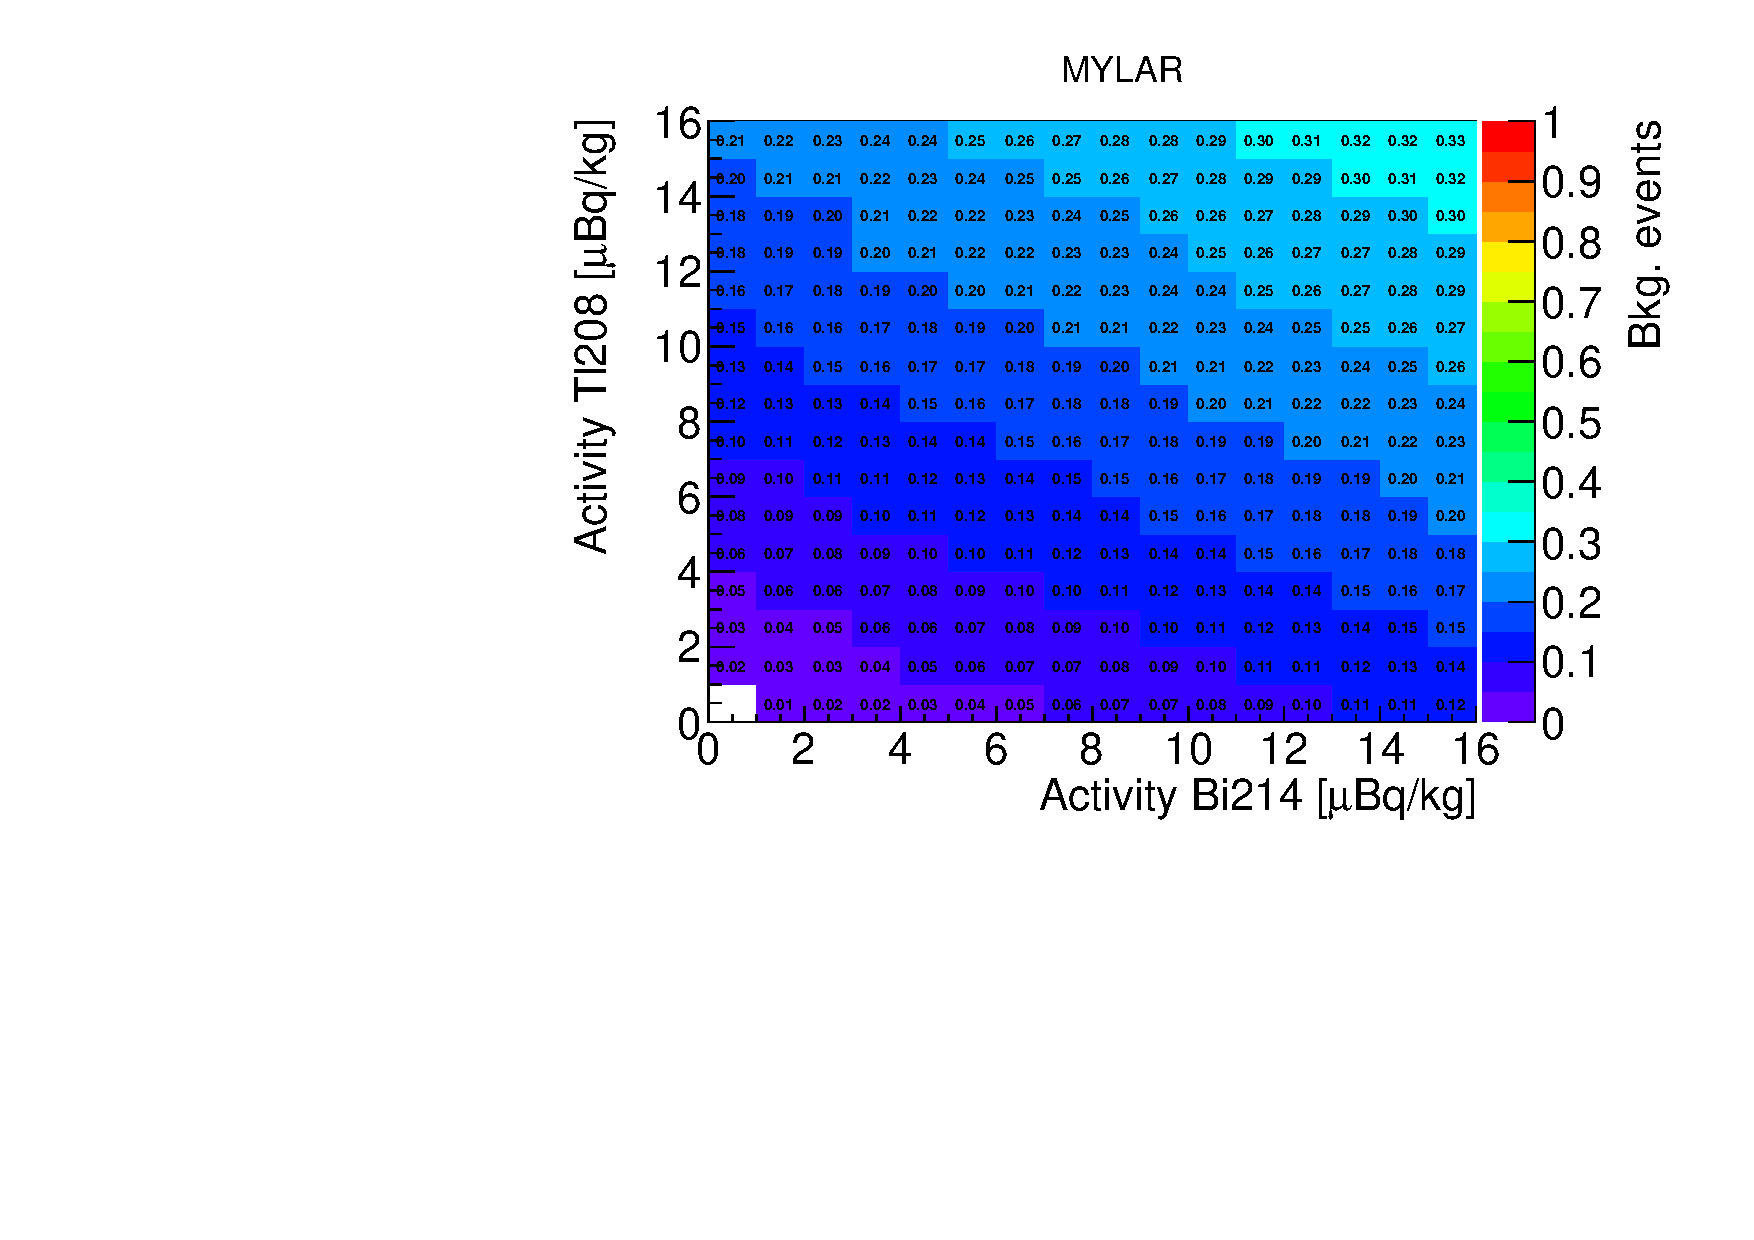
\includegraphics[scale=0.5]{pictures/Chap4/MYLAR_no2nu.pdf}
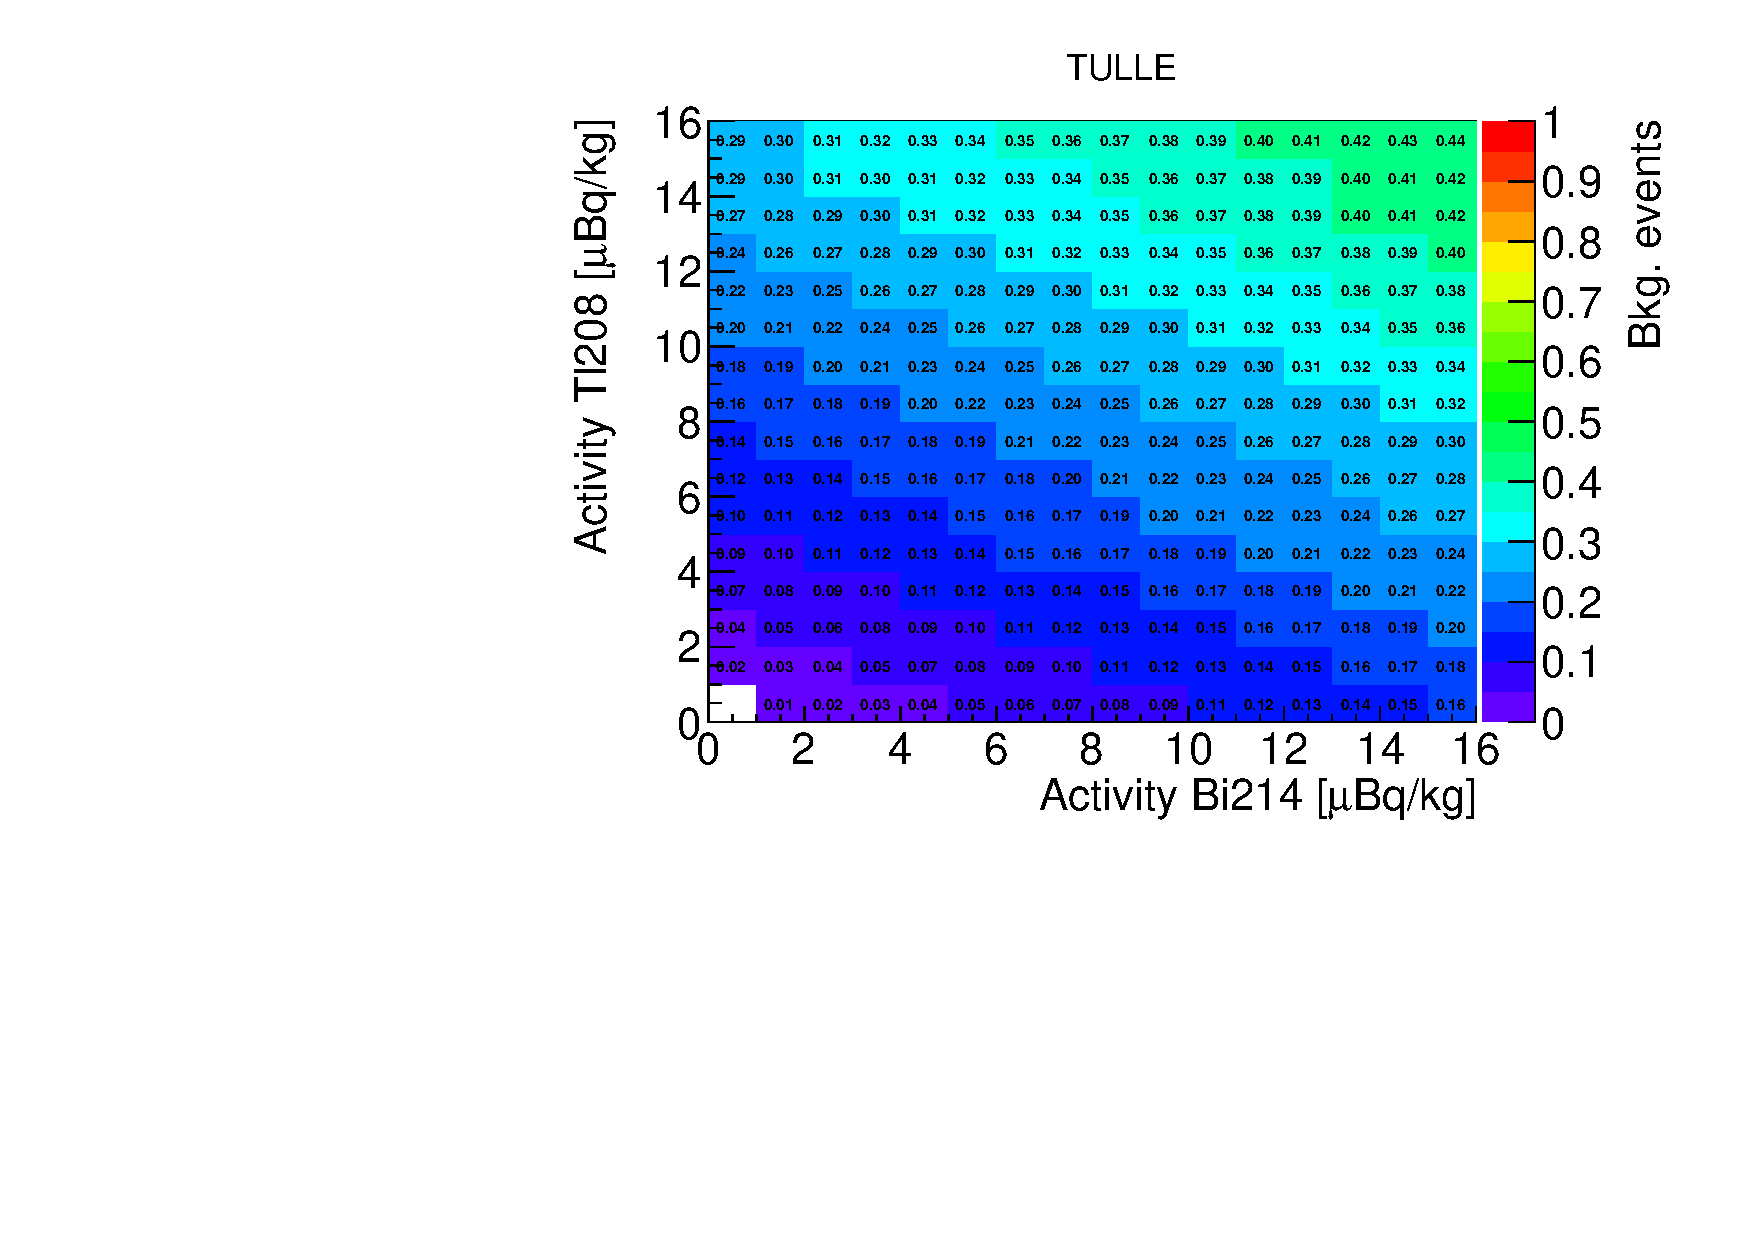
\includegraphics[scale=0.5]{pictures/Chap4/TULLE_no2nu.pdf}
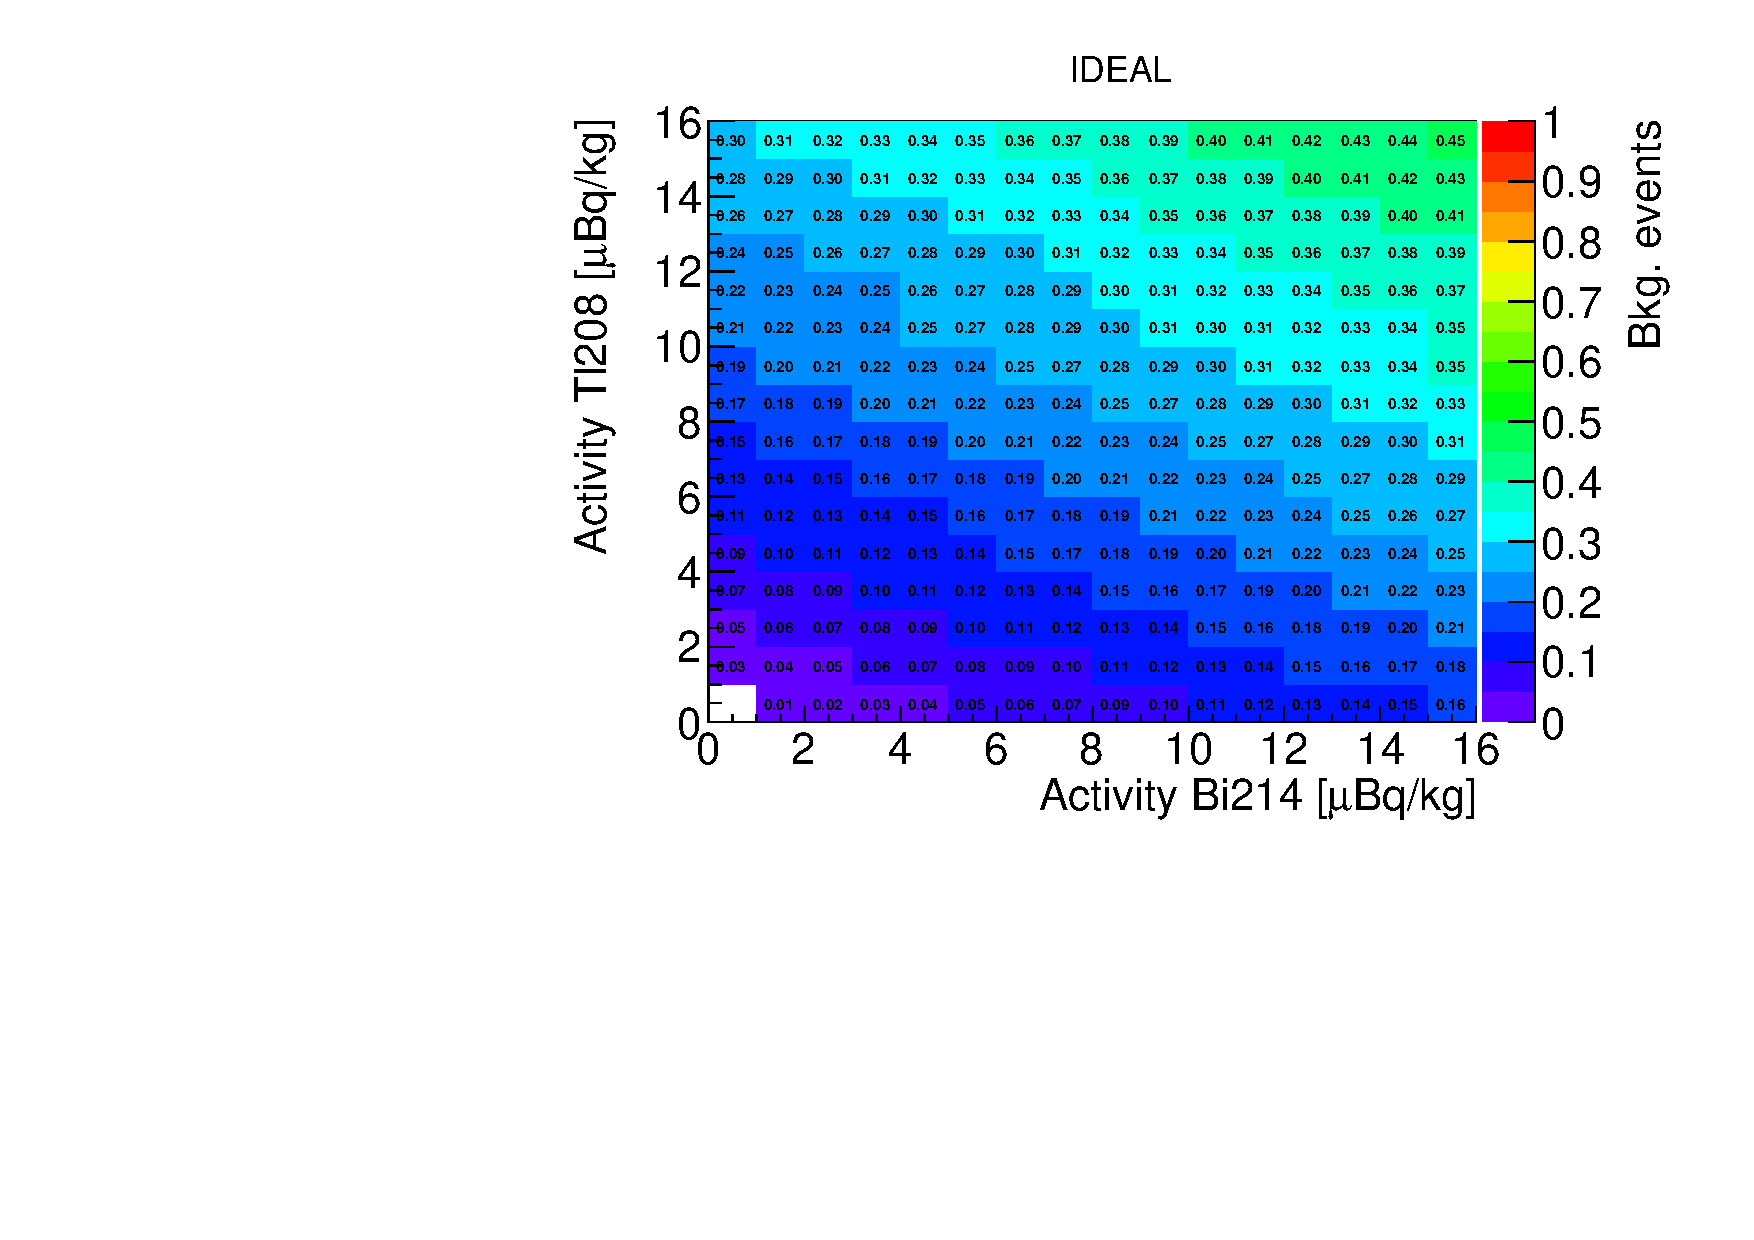
\includegraphics[scale=0.5]{pictures/Chap4/IDEAL_no2nu.pdf}
\label{Nbkg_3designs}
\caption{Expected number of total (2$\nu\beta\beta$ + $^{\text{208}}$Tl + $^{\text{214}}$Bi) background events as a function of the $^{\text{208}}$Tl and the $^{\text{214}}$Bi activity in the source foil for an exposure of 21 kg$\times$y. Top: MYLAR. Center: TULLE. Bottom: IDEAL}
\end{figure}


\begin{figure}[h!]
\centering
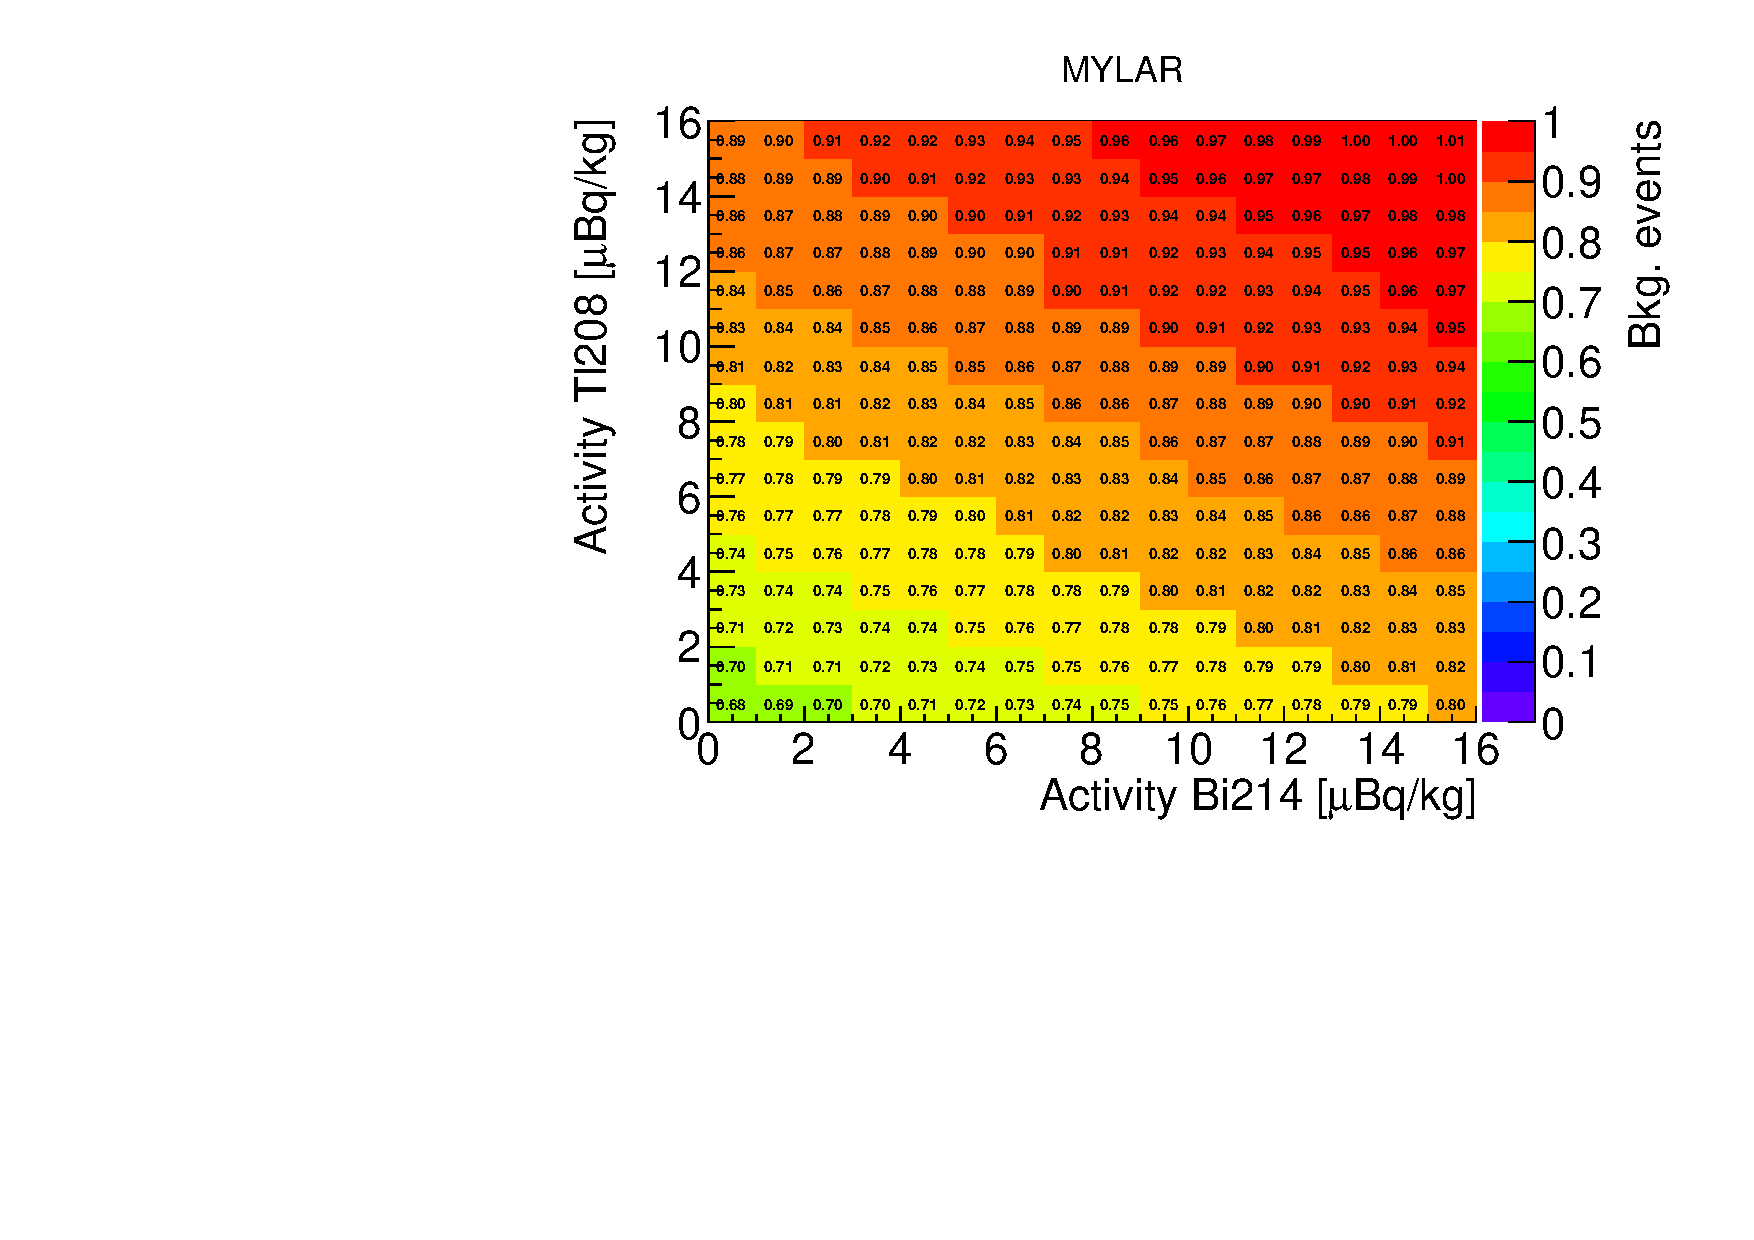
\includegraphics[scale=0.5]{pictures/Chap4/MYLAR_all.pdf}
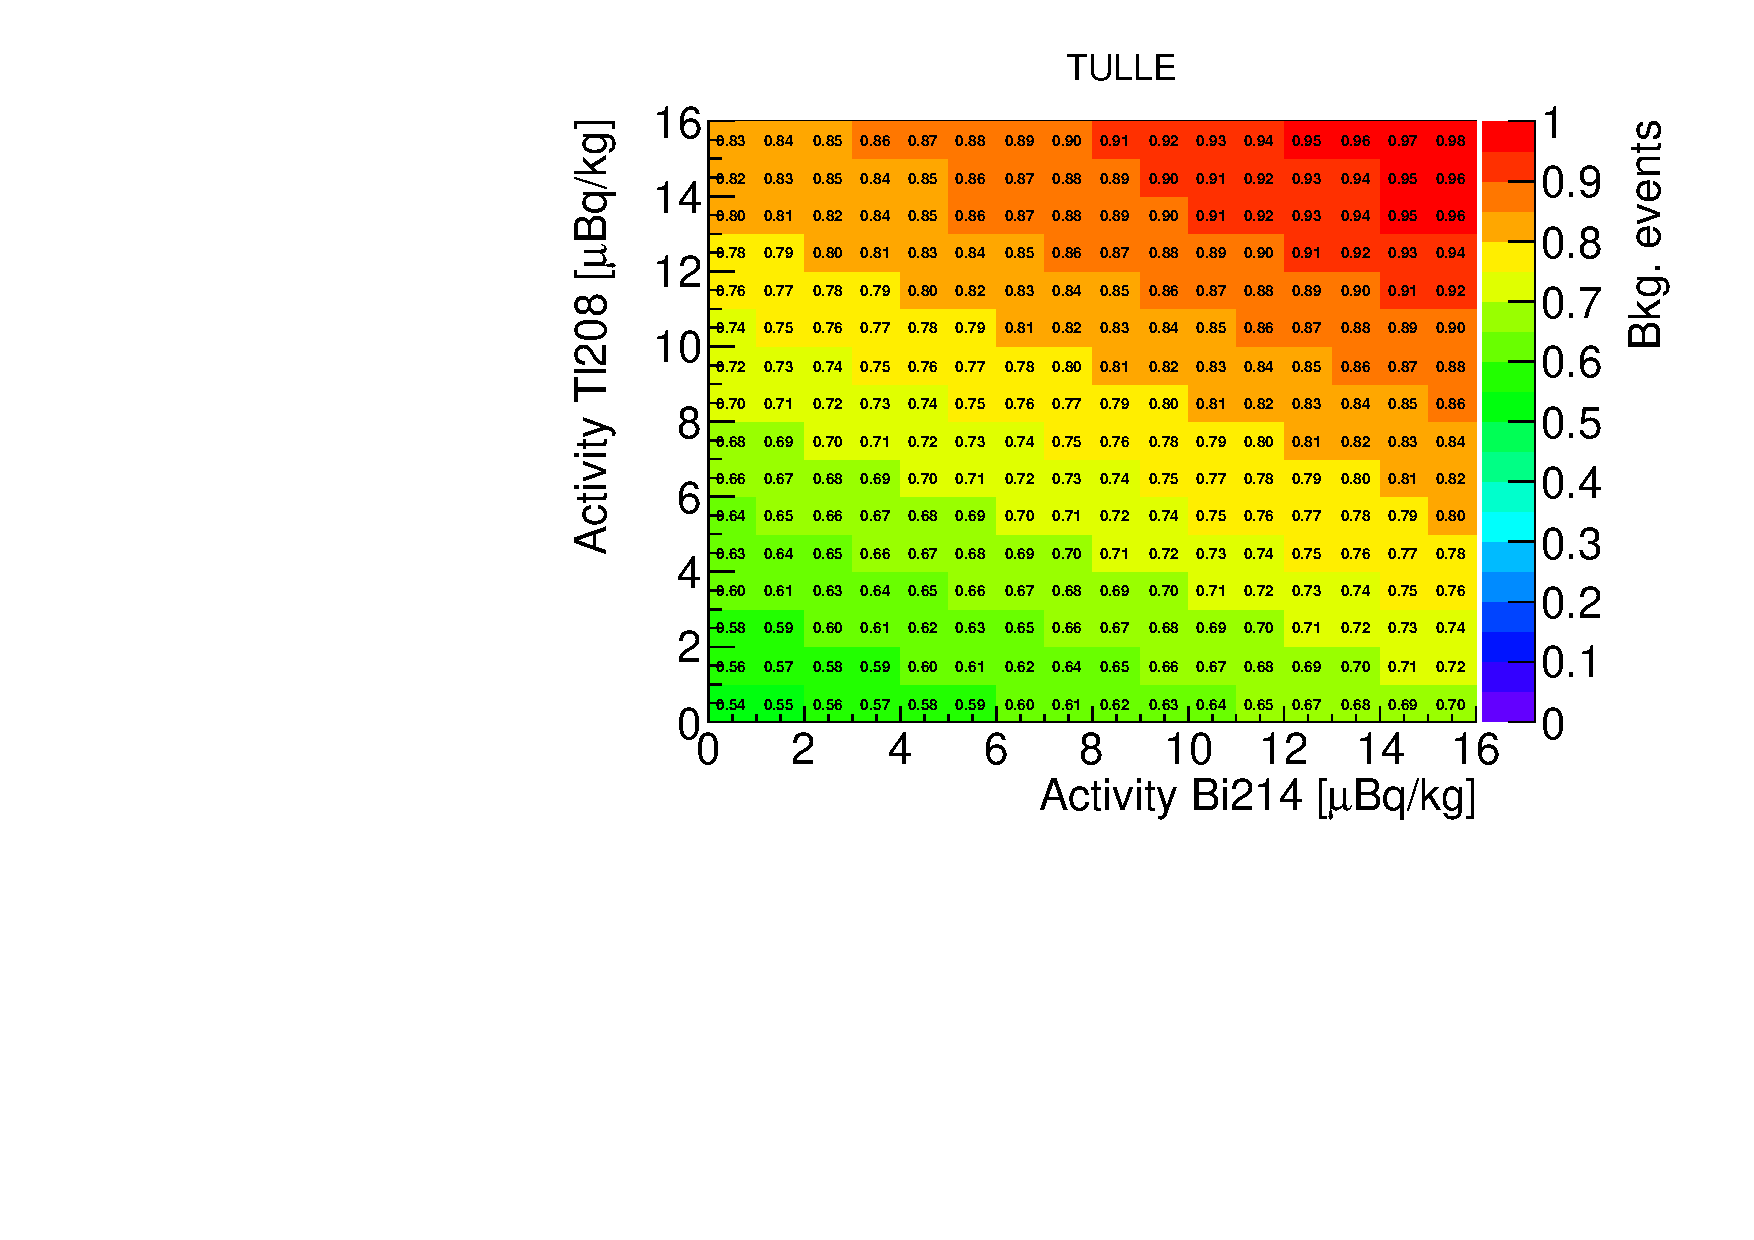
\includegraphics[scale=0.5]{pictures/Chap4/TULLE_all.pdf}
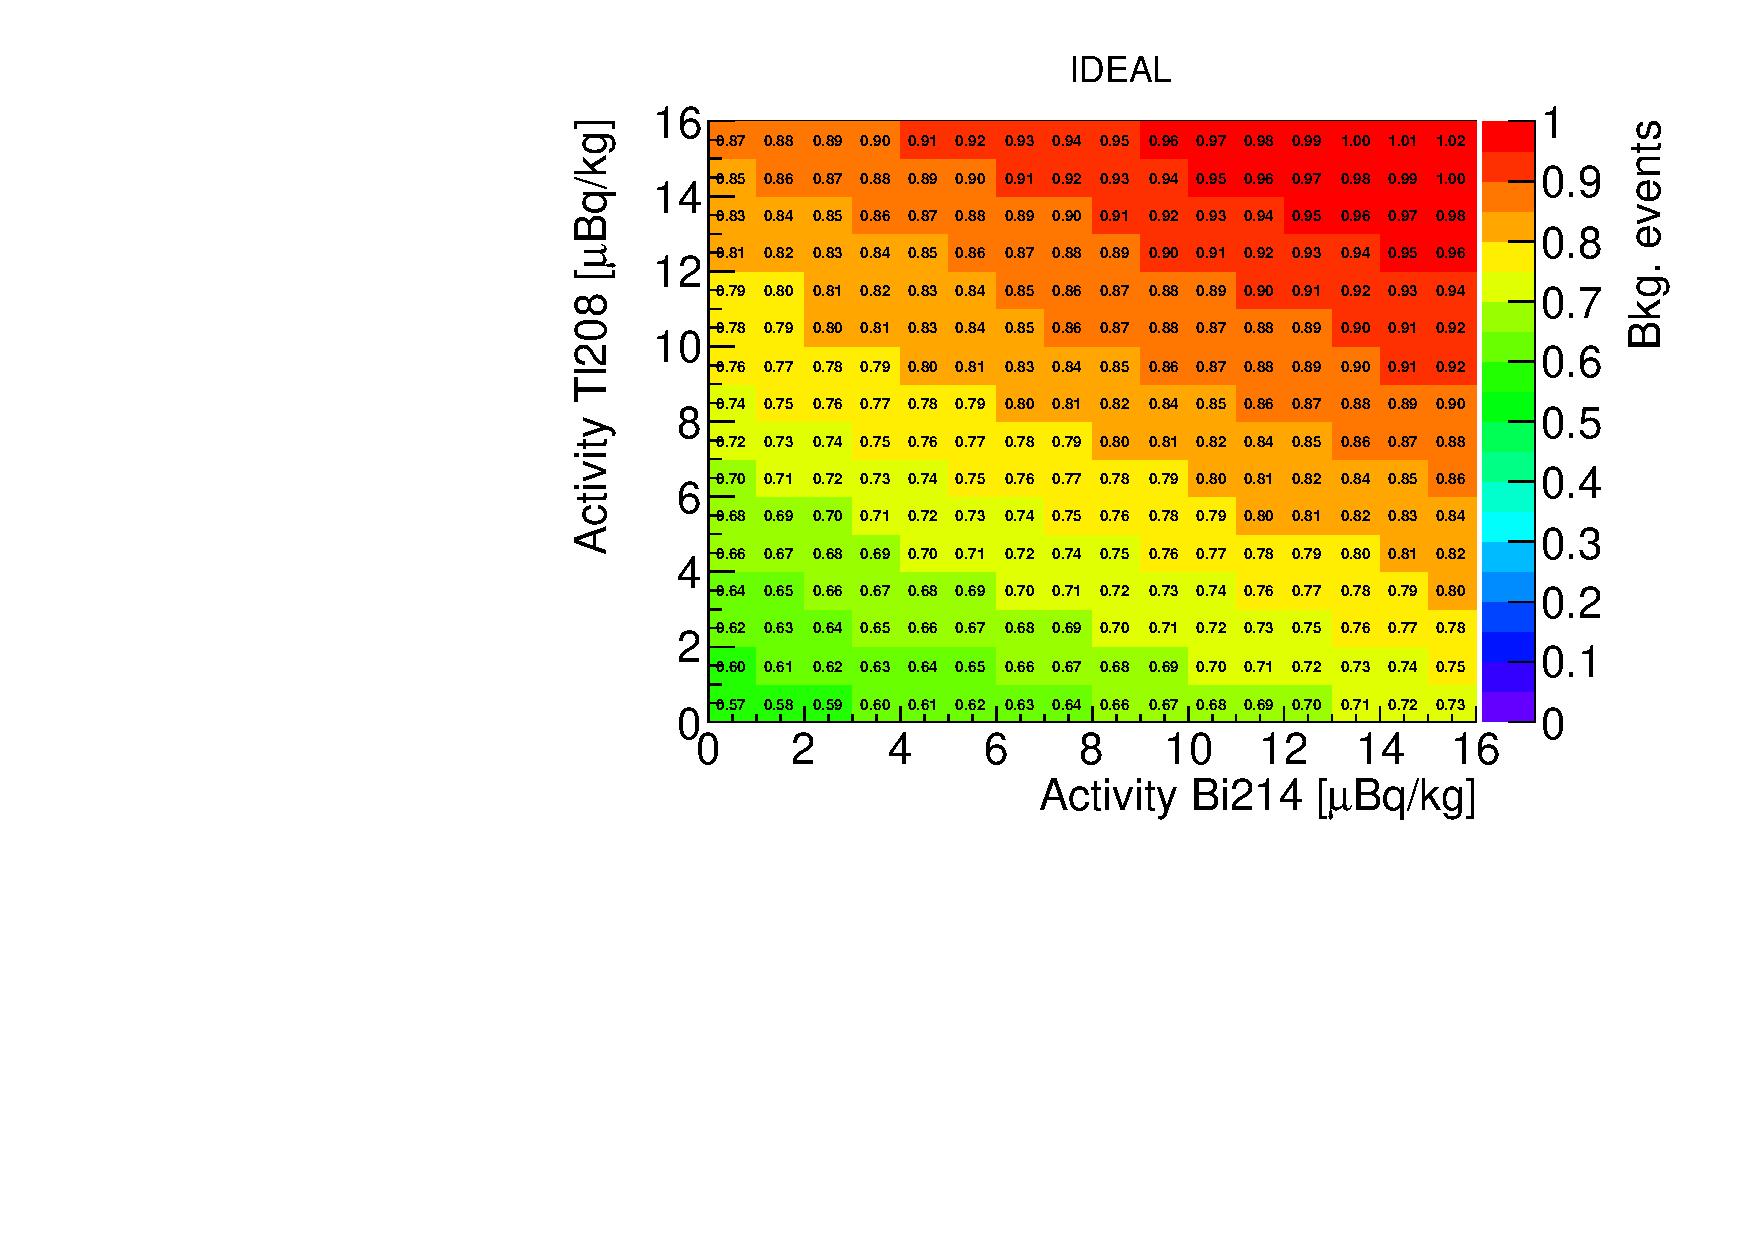
\includegraphics[scale=0.5]{pictures/Chap4/IDEAL_all.pdf}
\label{Nbkg_3designsTl208Bi214}
\caption{Expected number of $^{\text{208}}$Tl and $^{\text{214}}$Bi background events as a function of their activity in the source foil for an exposure of 21 kg $\times$ y as expected for the SuperNEMO demonstrator. Top: MYLAR. Center: TULLE. Bottom: IDEAL}
\end{figure}


\FloatBarrier


\subsection{Sensitivity vs. foil designs}\label{sec:SensitivityVsDesign}


\NI Table~\ref{Tab:SNperformanceDiffDesign} summarises the performances achievable with the SuperNEMO demonstrator module with respect to the source foil design, considering an exposure of 21 kg$\times$y. The signal and background p.d.f obtained in Section~\ref{sec:EventsEnergyDistribution} have been normalised to the $^{\text{208}}$Tl and the $^{\text{214}}$Bi activities measured by BiPo and summarised in Table~\ref{tab:MeasuredBiPoAndDensity}. The label IDEAL$^\star$ refers to IDEAL design case in which the background p.d.f. are normalised to the target radio-purity level of SuperNEMO. Figure~\ref{Sens2D-3designs} shows the result of the sensitivity scan w.r.t. the energy edges of the R.O.I.


\begin{table}[h!]
\centering
\begin{tabular}{c|c|c|c|c}
\toprule
Design & R.O.I [keV] & $\epsilon_{\text{0}\nu}$ [\%] & bkg. [cts.] &   T$_{\text{1/2}}^{\text{0}\nu}$ [$\times$ 10$^{\text{24}}$~y] \\[0.1cm]
\hline
IDEAL$^{\star}$ & [2720 ; 3060] & 17.44 $\pm$ 0.04 & 0.7 $\pm$ 0.1 & 6.12 \\  [0.1cm]
\hline
IDEAL           & [2720 ; 3060] & 17.44 $\pm$ 0.04 & 1.3 $\pm$ 0.1 & 5.34 \\  [0.1cm]
\hline
TULLE           & [2720 ; 3020] & 16.98 $\pm$ 0.04 & 2.3 $\pm$ 0.1 & 4.47 \\  [0.1cm]
\hline
MYLAR           & [2720 ; 3000] & 16.44 $\pm$ 0.04 & 2.1 $\pm$ 0.1 & 4.50 \\  [0.1cm]
\bottomrule
\end{tabular}
\caption{SuperNEMO demonstrator performance for different source foil designs.}
\label{Tab:SNperformanceDiffDesign}
\end{table}


\begin{figure}[h!]
\centering
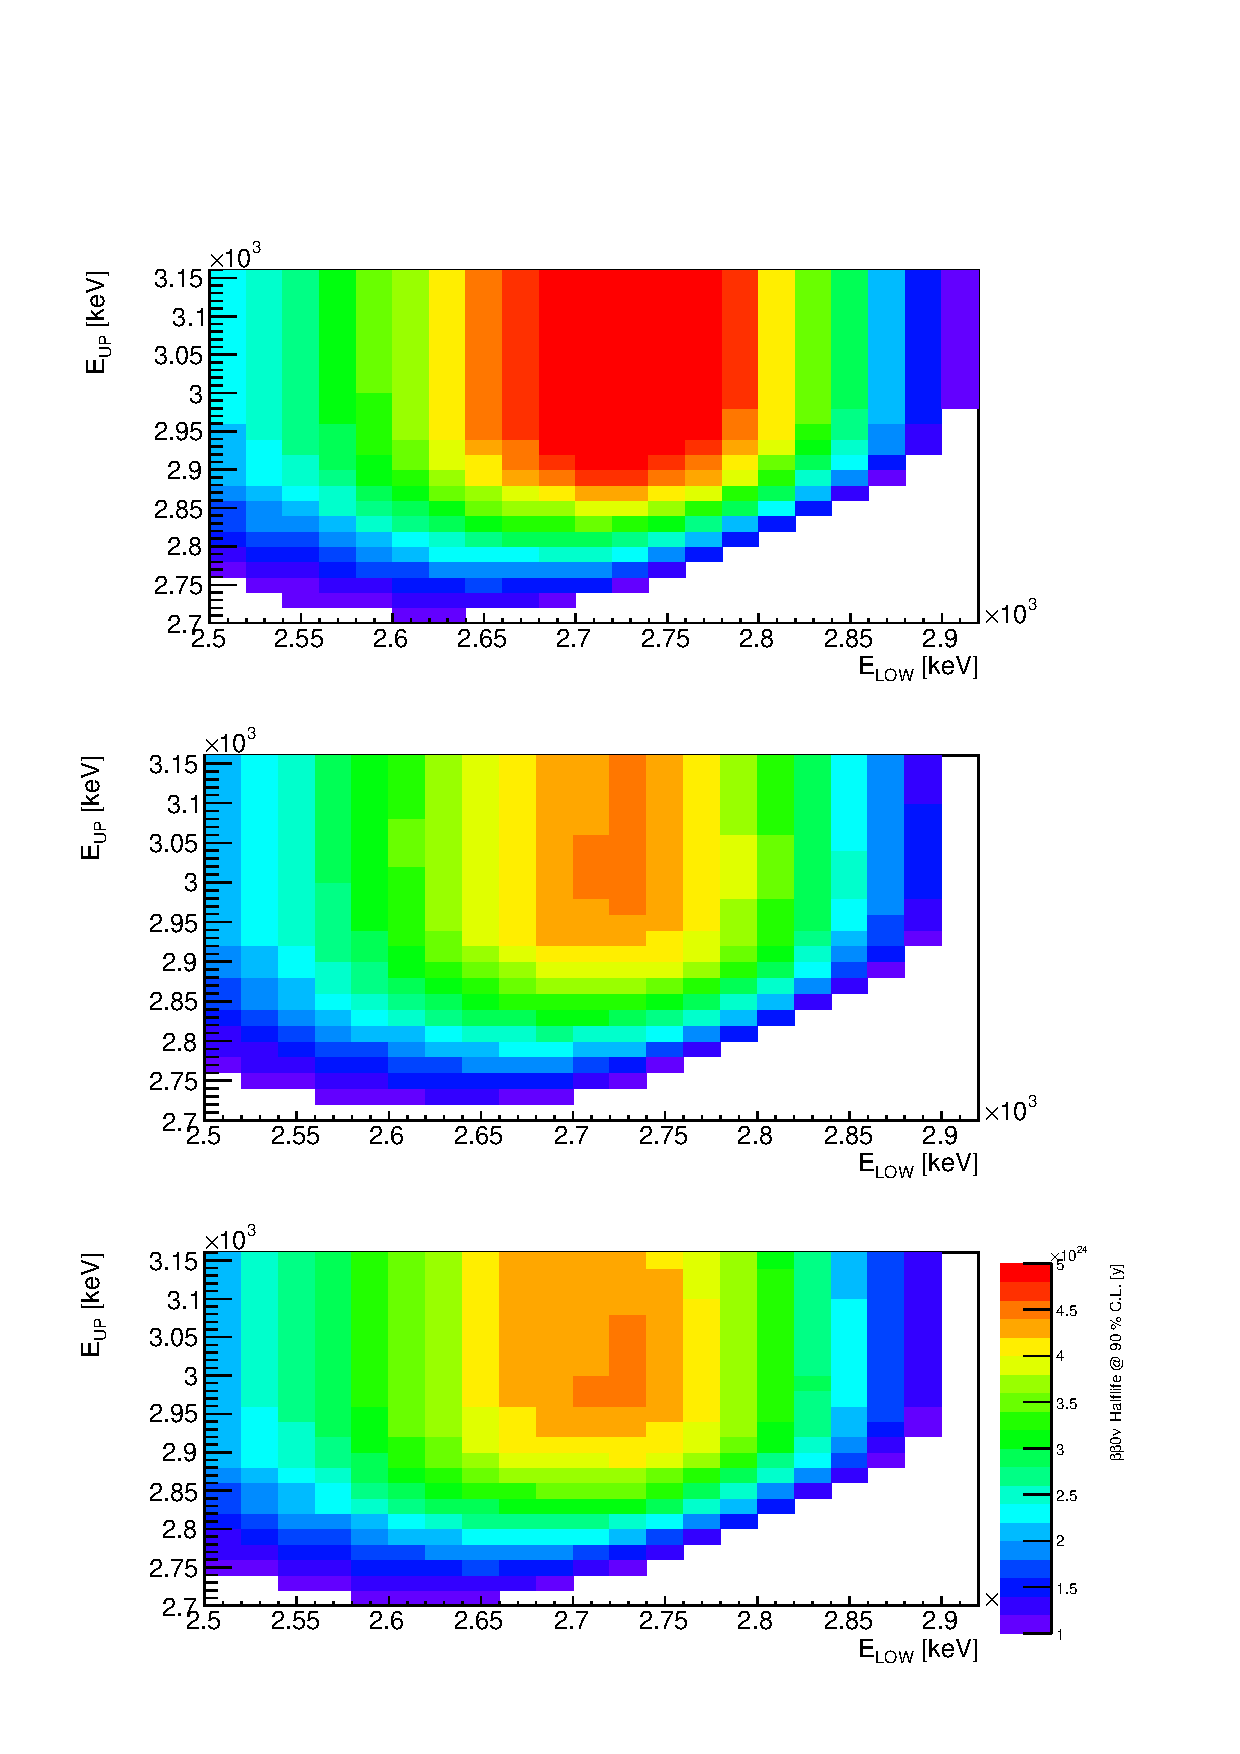
\includegraphics[scale=0.7]{pictures/Chap4/Sensitivity3Designs.pdf}
\caption{SuperNEMO demonstrator sensitivity for different source foil designs. Top: IDEAL. Center: TULLE. Bottom: MYLAR}
\label{Sens2D-3designs}
\end{figure}


\bigskip


\NI As discussed in Section~\ref{sec:EventsEnergyDistribution} the design of the source foil does not have a strong impact on the shape of the signal and background energy distributions. Nevertheless, the different activities of the material considered for the foil production and their mass fraction with respect to the $^{\text{82}}$Se affect in a non negligible way the performance of SuperNEMO. The performances obtained with the TULLE and MYLAR designs are compatible within~3\% but descrease  by approximately 16\% compared to the IDEAL design. Figure~\ref{SensVsExposure3Designs} shows the extrapolation of the SuperNEMO sensitivity beyond the exposure expected for the demonstrator module, up to 1000 kg$\times$y.


\begin{figure}[h!]
\centering
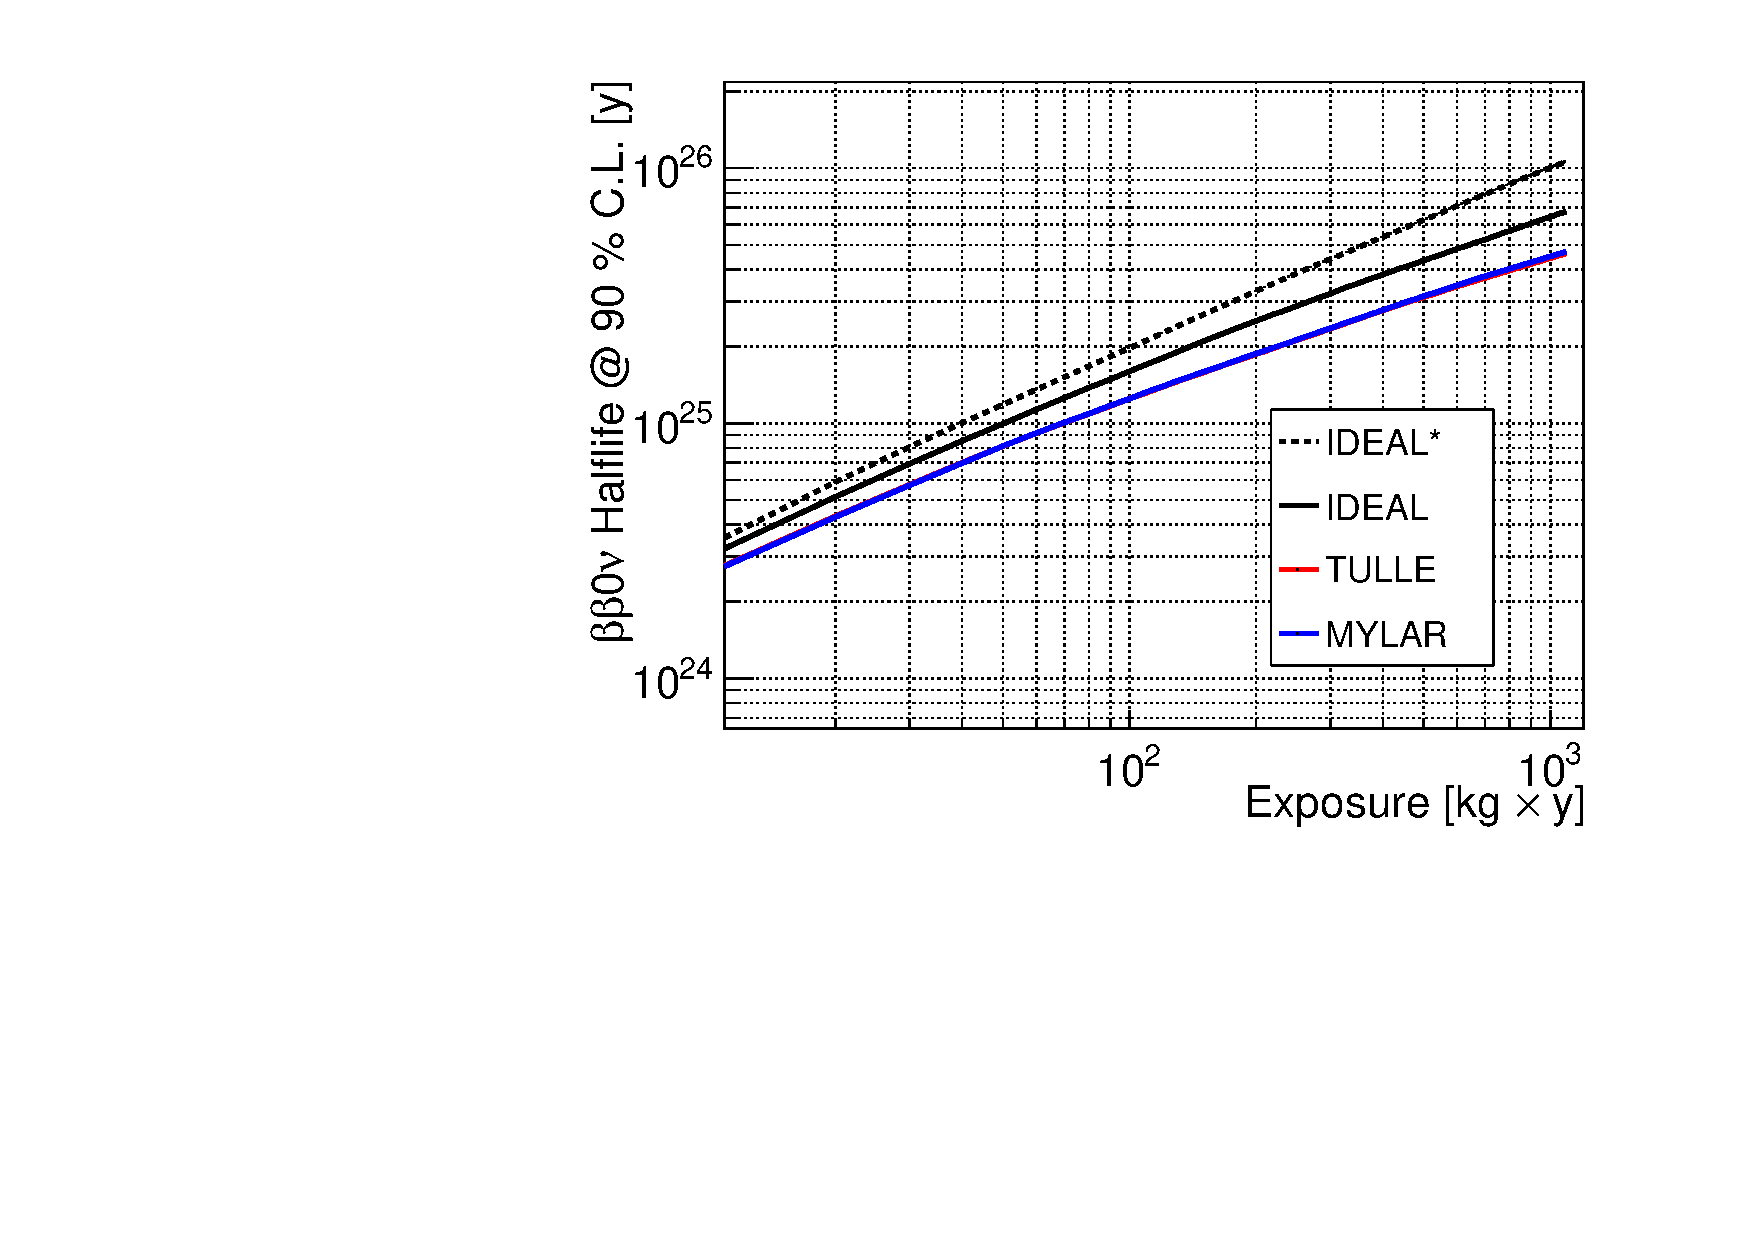
\includegraphics[scale=0.75]{pictures/Chap4/SensVsExposure.pdf}

\caption{SuperNEMO 0$\nu\beta\beta$ half-life limit at 90\% C.L. as a function of the exposure for the different source foil designs. The dotted line refers to the IDEAL design of the foil in which the backgrounds are normalised to the target radio-purity level of SuperNEMO.}
\label{SensVsExposure3Designs}
\end{figure}




%\begin{table}
%\centering
%\begin{tabular}{c|c|c|c|c}
%\toprule
%Design & R.O.I [keV] & $\epsilon_{\text{0}\nu}$ [\%] & bkg. [cts.] &   T$_{\text{1/2}}^{\text{0}\nu}$ [$\times$ 10$^{\text{24}}$~y] \\[0.1cm]
%\hline
%IDEAL           & [2700 ; 2980] & 19.47 $\pm$ 0.04 & 4.9 $\pm$ 0.2 & 3.8 \\  [0.1cm]
%\hline
%TULLE           & [2700 ; 3000] & 17.20 $\pm$ 0.04 & 6.3 $\pm$ 0.2 & 3.5 \\  [0.1cm]
%\hline
%MYLAR           & [2700 ; 3980] & 17.68 $\pm$ 0.04 & 6.0 $\pm$ 0.2 & 3.4 \\  [0.1cm]
%\bottomrule
%\end{tabular}
%\caption{SuperNEMO demonstrator performance in 21 kg$\times$y considering an additional contamination of 100 $\mu$Bq/kg both in 208 Tl and 214 Bi to mimic the effect of an high contamination from 82 Se powder.}
%\label{SNperformanceDiffDesign2}
%\end{table}


\FloatBarrier


\subsection{Optimising the amount of PVA}\label{sec:OptimisingAmountPVA}


\NI The amount of PVA introduced in the foil during its fabrication has an impact on the its thickness and its density as shown in Figure~\ref{Tab:PamameterAmountPVA}. The amount of PVA also modifies the shape of the signal and background p.d.f as shown in Figure~\ref{SpectrumPVA} as well as the background level. Table~\ref{Tab:AmountOfPVA} summarizes the results of the performance study as a function of the amount of PVA for the TULLE design. Best performances are obtained without PVA, but this scenario is not technically feasible since the $^{\text{82}}$Se foil will not be resistant enough. A TULLE foil containing 5\% of PVA would still be compatible with the IDEAL design within 10\%, but it would be very hard to produce, as observed during the R\&D tests at LAPP. From the technical point of view, a fraction of 10-15\% of PVA seems more reasonable and would allow of achieving performance compatible with the MYLAR design within 10\%.


\bigskip	


\begin{figure}[h!]
\centering
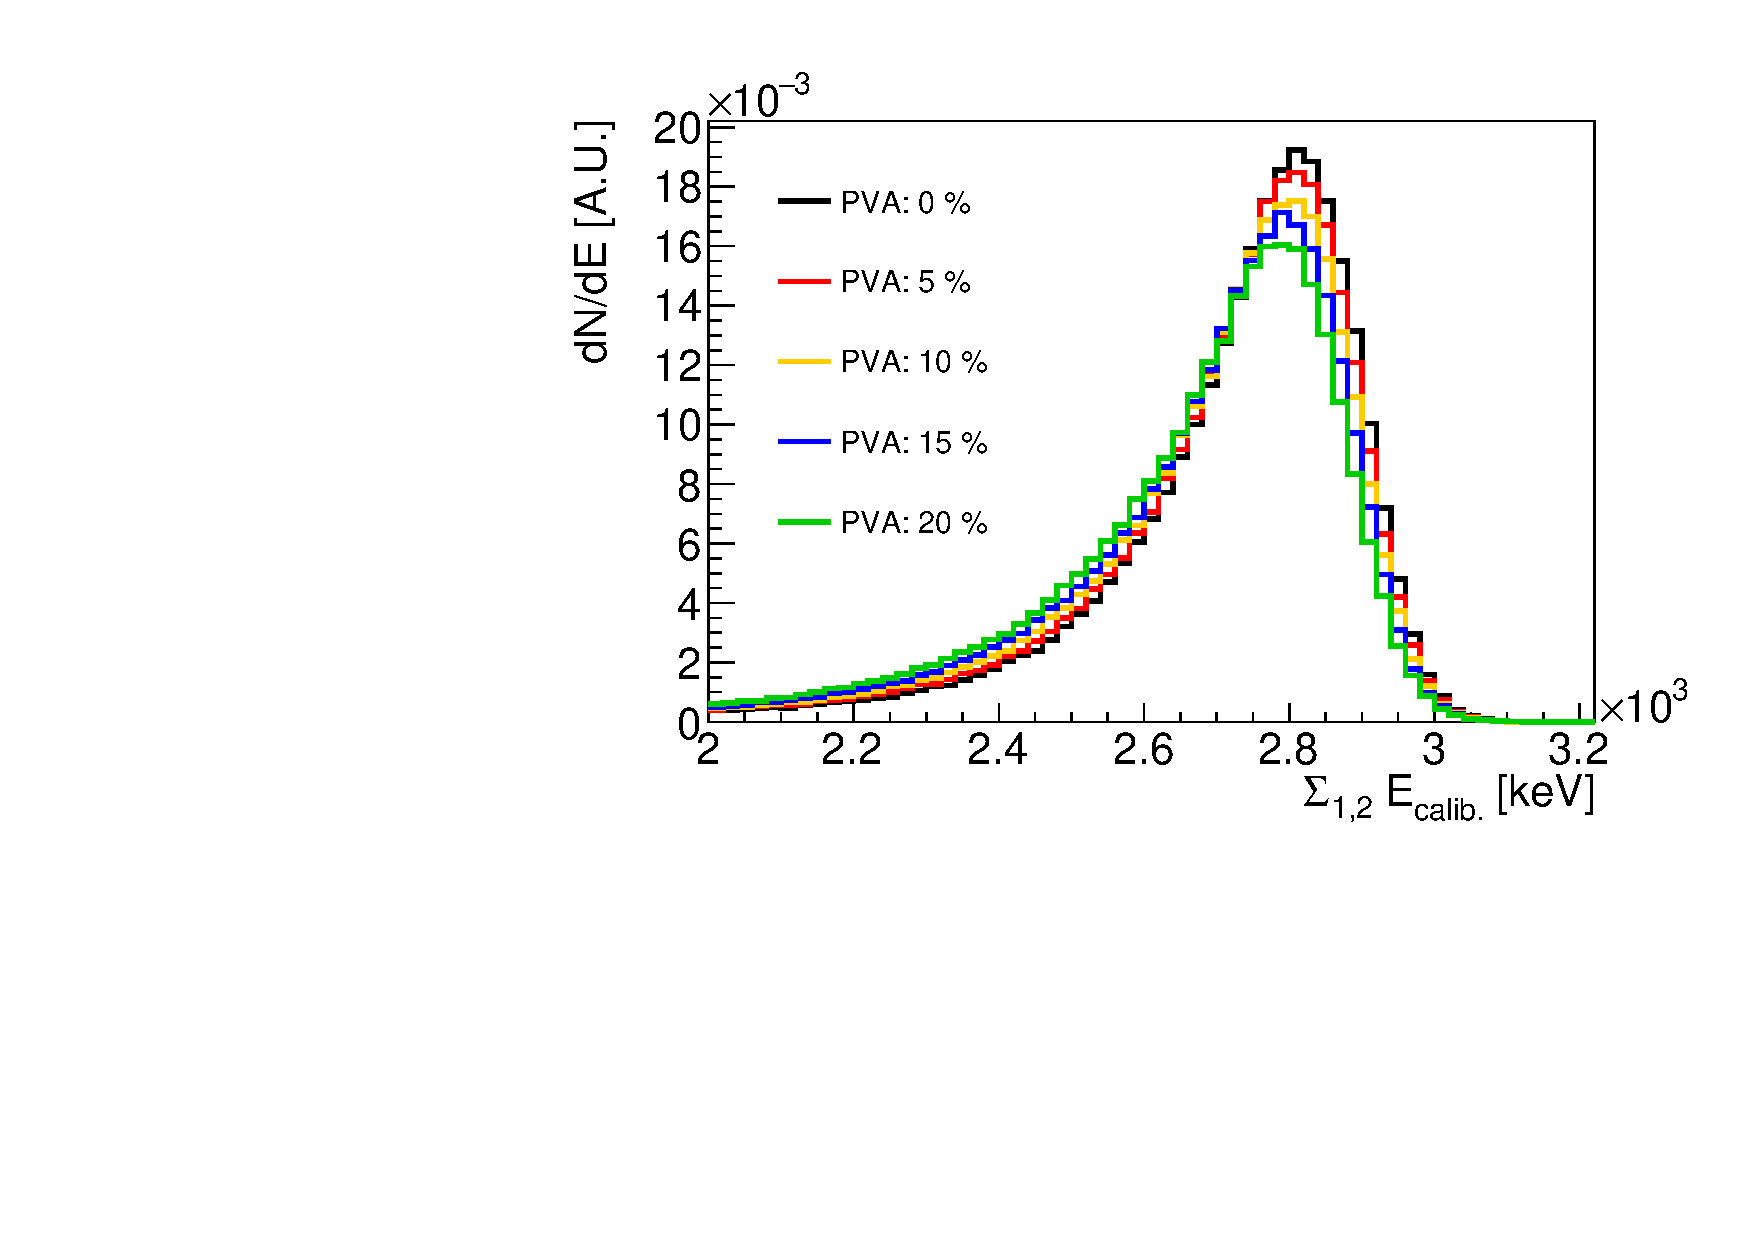
\includegraphics[scale=0.6]{/home/lenoblet-local/Bureau/Thesis/pictures/Chap4/PVAfraction.pdf}
\caption{0$\nu\beta\beta$ p.d.f. with TULLE foils containing different amounts of PVA. The increased amount of PVA shifts the p.d.f. toward lower energies, due to an increased e energy loss in a thicker foil.}
\label{SpectrumPVA}
\end{figure}


\begin{table}
\centering
\begin{tabular}{c|c|c|c|c|c|c|c}
\toprule 
f$_{\text{Se}}$ & f$_{\text{PVA}}$ & f$_{\text{Support}}$ & a & $\rho$ & t & A ($^{\text{214}}$Bi) & A ($^{\text{208}}$Tl) \\ [0.1cm] 
[-] & [-] & [-] & [mg/cm$^\text{2}$] & [g/cm$^\text{3}$] & [$\mu$m] & [$\mu$Bq] & [$\mu$Bq] \\[0.1cm]
\hline 
0.986 & 0.00 & 0.014 & 50.7 & 3.17 & 160 & 10.2 & 6.1 \\ [0.1cm]
\hline 
0.937 & 0.05 & 0.013 & 53.4 & 3.08 & 173 & 72.7 & 9.6 \\ [0.1cm]
\hline 
0.888 & 0.10 & 0.012 & 56.3 & 2.98 & 189 & 142.0 & 13.5 \\ [0.1cm]
\hline 
0.838 & 0.15 & 0.012 & 59.6 & 2.89 & 206 & 219.8 & 17.8 \\ [0.1cm]
\hline 
0.789 & 0.20 & 0.011 & 63.4 & 2.80 & 227 & 306.9 & 22.6 \\ [0.1cm]
\bottomrule 
\end{tabular} 
\caption{Parameters of TULLE foils containing different amounts of PVA.}
\label{Tab:PamameterAmountPVA}
\end{table}


\begin{table}
\centering
\begin{tabular}{c|c|c|c|c}
\toprule
f$_{\text{PVA}}$ & R.O.I [keV] & $\epsilon_{\text{0}\nu}$ [\%] & bkg. [cts.] &   T$_{\text{1/2}}^{\text{0}\nu}$ [$\times$ 10$^{\text{24}}$~y] \\[0.1cm]
\hline
0.00 & [2720 ; 3040] & 17.84 $\pm$ 0.04 & 0.9 $\pm$ 0.1 & 6.03 \\ [0.1cm]
\hline
0.05 & [2700 ; 3020] & 18.31 $\pm$ 0.04 & 2.0 $\pm$ 0.1 & 5.01 \\ [0.1cm]
\hline
0.10 & [2720 ; 3020] & 16.98 $\pm$ 0.04 & 2.3 $\pm$ 0.1 & 4.47 \\ [0.1cm]
\hline
0.15 & [2700 ; 2980] & 16.27 $\pm$ 0.04 & 3.3 $\pm$ 0.2 & 3.85 \\ [0.1cm]
\hline
0.20 & [2680 ; 3020] & 16.51 $\pm$ 0.04 & 5.7 $\pm$ 0.3 & 3.26 \\ [0.1cm]
\bottomrule
\end{tabular}
\caption{SuperNEMO performances with TULLE foils containing different amounts of PVA.}
\label{Tab:AmountOfPVA}
\end{table}


\FloatBarrier


\subsection{Foil uniformity}\label{sec:FoilUniformity}


\NI The thickness of the source foil impacts the energy losses of the out-coming particles worsening the resolution on the energy measurement. For similar reasons, the thickness also impacts also the probability of observing 2e events from the beta decay of $^{\text{208}}$Tl and $^{\text{214}}$Bi. During the production of the source foil, the $^{\text{82}}$Se and the PVA paste is poured on a dedicated support and spread uniformly over the surface. Since the process is performed manually, a non uniform deposition of the paste may happen. This will cause a non uniform thickness over the foil length affecting the performance of the SuperNEMO demonstrator in terms of background level and sensitivity. For this reason it is important to study such effects in order to define the acceptable level of uniformity of the source foil.


\subsubsection{Signal and background vs foil thickness}


\NI Signal and background events have been simulated considering a TULLE foil design containing 90\% of $^{\text{82}}$Se and 10\% of PVA. The reference thickness of 190~$\mu$m has been varied by $\pm$10\% and $\pm$20\%. For each foil thickness, the simulated sample consists of 10$^\text{6}$ 0$\nu\beta\beta$ events and 10$^\text{7}$ events for each background channel, 2$\nu\beta\beta$ , $^{\text{208}}$Tl and $^{\text{214}}$Bi. The expected energy spectra of the 2e channel are shown in Figure~\ref{ThicknessSourceFoil} for the different thicknesses. It clearly appears looking at the 0$\nu\beta\beta$ (top left) and the 2$\nu\beta\beta$ (top right) spectra of Figure~\ref{ThicknessSourceFoil} that the overall effect is a worsening of the energy resolution (increasing of the 0$\nu\beta\beta$ peak width) and a shift of the events towards lower energies due to an increase of the energy lost within the foil. Table~\ref{tab:SignalBkgDifferentThickness} summarises the impact of the source foil thickness on the selection efficiency for the signal and the backgrounds. The selection efficiency being defined as the fraction of events satisfying the simple selection criteria of two reconstructed negative tracks hitting two calo blocks with a total energy deposition in [2700; 3000] MeV, defined as the ROI maximising the sensitivity to T$_{\text{1/2}}$. The total background level and the best sensitivity obtained in the ROI are summarised in Table~\ref{Tab:ThicknessInfluence}.



\begin{table}
\centering
\begin{tabular}{c|c|c|c|c|c}
\toprule
t & Density & $\epsilon_{\text{0}\nu}$ & $\epsilon_{\text{2}\nu}$ & $\epsilon_{\text{Tl}}$ & $\epsilon_{\text{Tl}}$ \\[0.1cm] 
[$\mu$m] & [mg/cm$^\text{2}$] & [\%] & $\times$10$^{-\text{5}}$[\%] & $\times$10$^{-\text{3}}$[\%] & $\times$10$^{-\text{3}}$[\%] \\[0.1cm]
\hline
150 & 44.7 & 19.58 $\pm$ 0.04 & 8.84 $\pm$ 0.05 & 3.2 $\pm$ 0.2 & 2.1 $\pm$ 0.1 \\
\hline
170 & 50.7 & 18.37 $\pm$ 0.04 & 7.92 $\pm$ 0.05 & 2.8 $\pm$ 0.2 & 1.9 $\pm$ 0.1 \\
\hline
190 & 56.6 & 17.25 $\pm$ 0.04 & 6.29 $\pm$ 0.05 & 3.0 $\pm$ 0.2 & 1.6 $\pm$ 0.1 \\
\hline
210 & 62.6 & 16.07 $\pm$ 0.04 & 5.59 $\pm$ 0.04 & 2.9 $\pm$ 0.2 & 1.6 $\pm$ 0.1 \\
\hline
230 & 68.5 & 14.95 $\pm$ 0.04 & 4.00 $\pm$ 0.04 & 3.1 $\pm$ 0.2 & 1.4 $\pm$ 0.1 \\
\bottomrule
\end{tabular}
\caption{Signal and background efficiencies for E$_\beta\beta$ in [2700; 3000] keV.}
\label{tab:SignalBkgDifferentThickness}
\end{table}


\begin{table}
\centering
\begin{tabular}{c|c|c}
\toprule
t [$\mu$m] & Bkg. [cts.] &  T$_{\text{1/2}}^{\text{0}\nu}$ [$\times$ 10$^{\text{24}}$~y] \\[0.1cm]
\hline
150 & 3.3 $\pm$ 0.2 & 4.63 \\[0.1cm]
170 & 3.0 $\pm$ 0.2 & 4.46 \\[0.1cm]
190 & 2.5 $\pm$ 0.1 & 4.41 \\[0.1cm]
210 & 2.4 $\pm$ 0.1 & 4.15 \\[0.1cm]
230 & 2.1 $\pm$ 0.1 & 4.01 \\[0.1cm]
\bottomrule
\end{tabular}
\caption{Background level and best sensitivity for E in [2700; 3000] keV.}
\label{Tab:ThicknessInfluence}
\end{table}


\begin{figure}[h!]
\centering
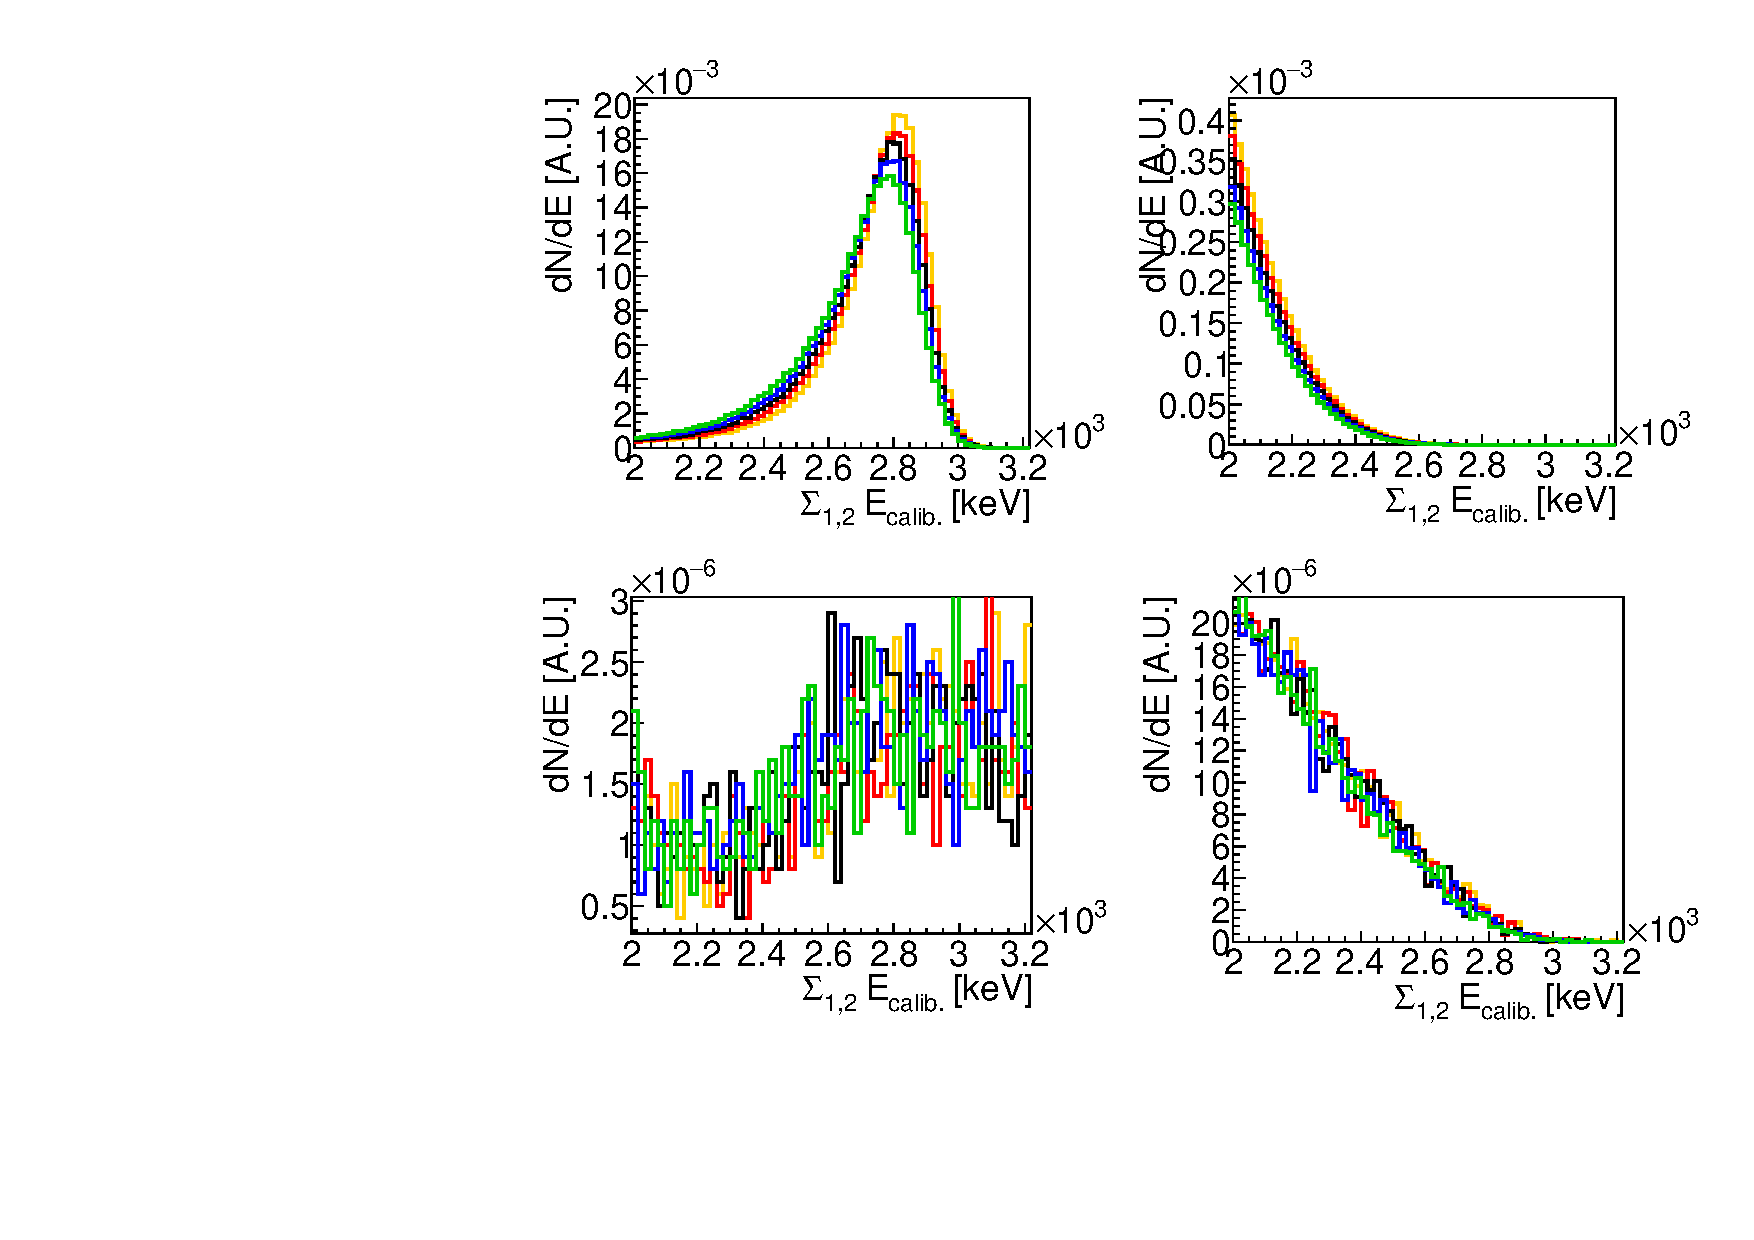
\includegraphics[scale=0.7]{pictures/Chap4/thickness.pdf}
\caption{Signal and background p.d.f. generated with different source foil thickness : 150 $\mu$m (yellow), 170 $\mu$m (red), 190 $\mu$m (black), 210 $\mu$m (blue), 220 $\mu$m (green)}
\label{ThicknessSourceFoil}
\end{figure}

\FloatBarrier


\subsubsection{Effects of the foil uniformity}


\NI To mimic the effect of a non uniform foil thickness, we consider a case in which half of the foil is, for example, +10\% thicker and the other half is -10\% thinner than the nominal value. The average thickness of such a foil is still the nominal value and the amount of $^{\text{82}}$Se + PVA paste required to produce it would be unchanged. The overall effect of such a non uniformity on a generic observable x is then obtained by averaging the same observable x$_+$ and x$_-$ obtained for the thicker and the thinner foil respectively. The relative comparison against the same observable obtained with the nominal thickness allows to obtain the systematic effect $\sigma$ due to the non uniformity :


\begin{equation}
\langle \text{x} \rangle = \text{x}_+ \left( \frac{\text{t}_+}{\text{t}_+ + \text{t}_-}  \right) + \text{x}_- \left( \frac{\text{t}_-}{\text{t}_+ + \text{t}_-}  \right) 
\end{equation}


\begin{equation}
\sigma_\text{x} = \frac{|\langle \text{x}\rangle - \text{x}|}{\text{x}}
\end{equation}


\bigskip


\NI The red and the blue histograms in Figure~\ref{SpectrumThickness} show the averaged spectra obtained varying the foil thickness by $\pm$10\% and $\pm$20\% respectively. The black histogram shows the expected spectra at the nominal thickness of 190 $\mu$m. Table~\ref{Tab:SystematicInfluence} shows the systematic effects on the signal and background selection efficiencies induced by a foil non uniformity for E$_{\beta\beta}$ in [2700; 3000] keV, where the best sensitivity is found.



\begin{figure}[h!]
\centering
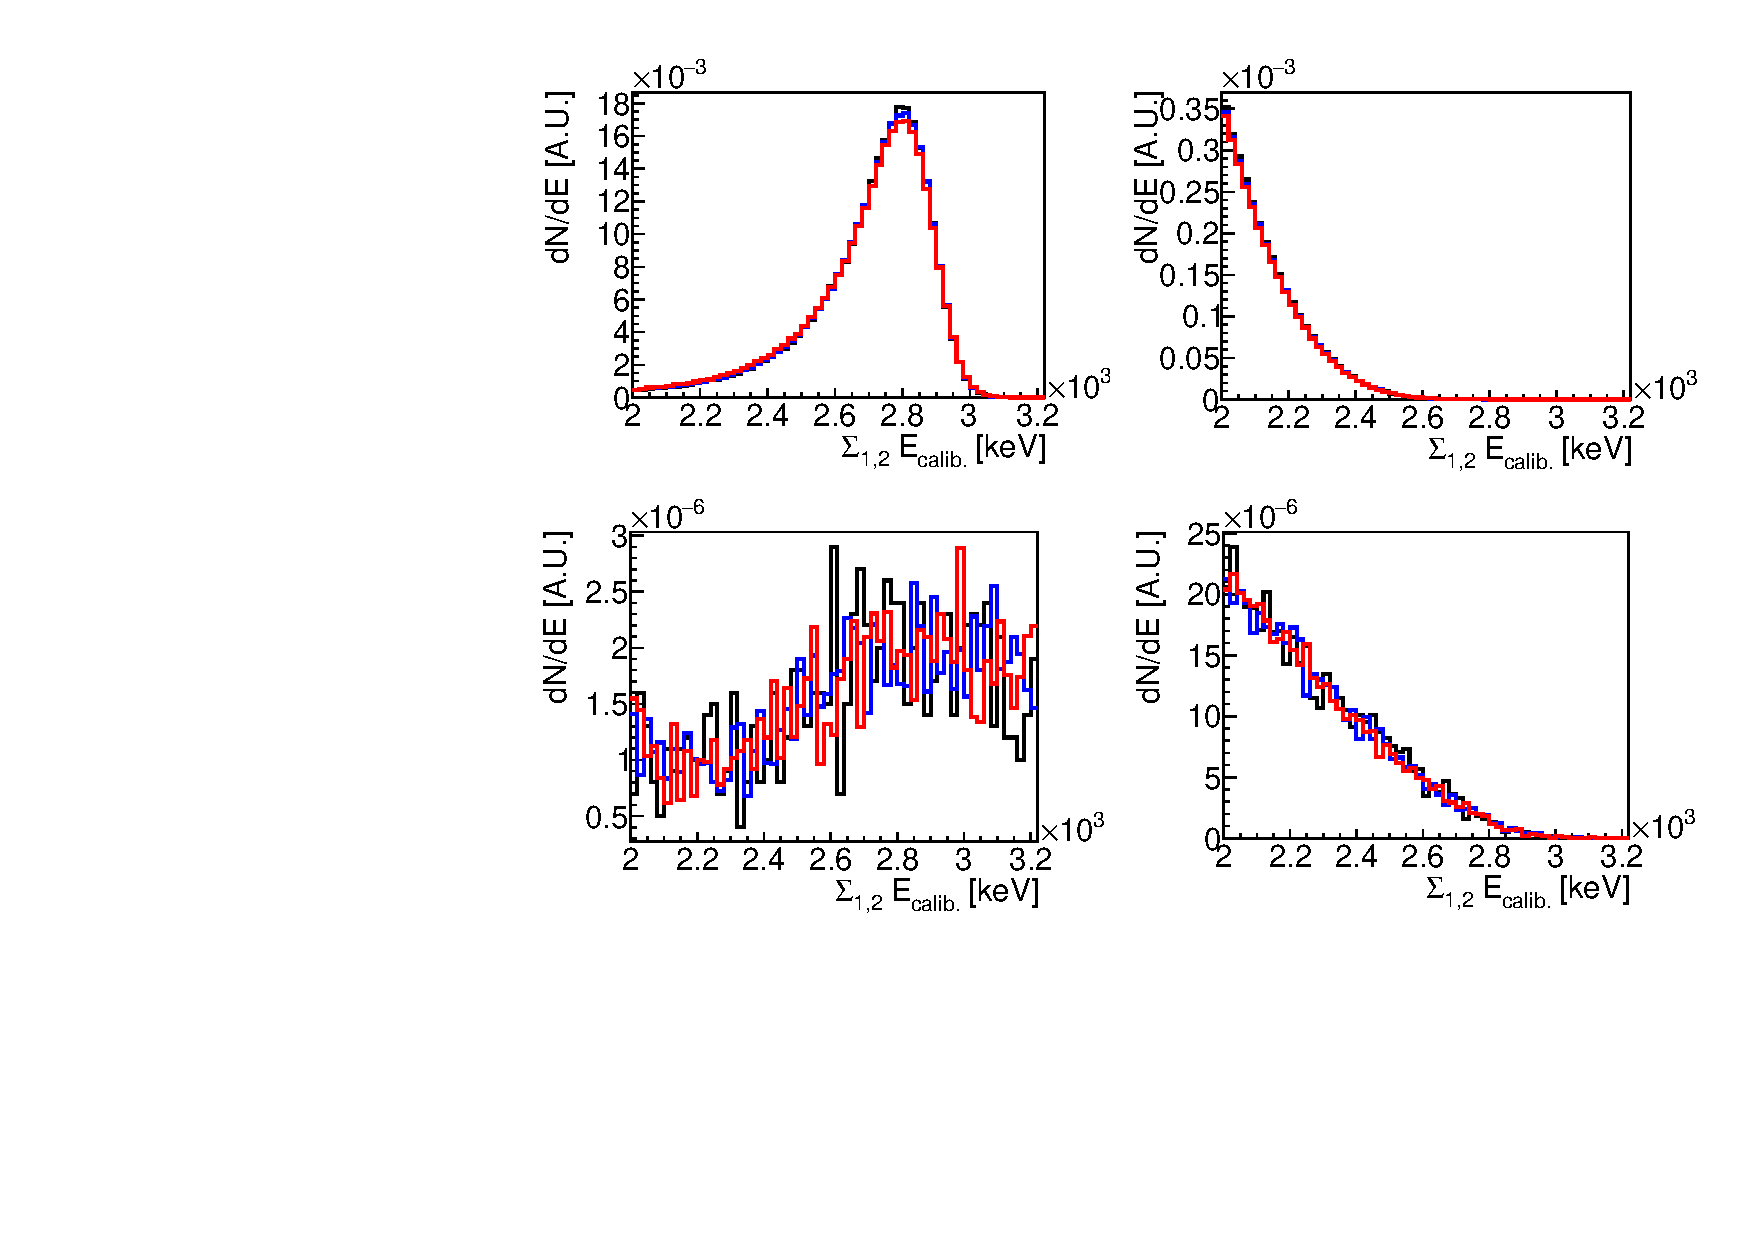
\includegraphics[scale=0.7]{pictures/Chap4/Syst.pdf}
\caption{The red and the blue histograms show the expected spectra by variating the foil thickness by $\pm$10\% and $\pm$20\% respectively. The black histogram shows the expected spectra at the nominal thickness of 190 $\mu$m.}
\label{SpectrumThickness}
\end{figure}


\begin{table}[h!]
\centering
\begin{tabular}{c|c|c|c|c|c}
\toprule
\multirow{2}{*}{Uniformity} & $\sigma_{\epsilon \text{0}\nu}$ & $\sigma_{\epsilon \text{2}\nu}$ & $\sigma_{\epsilon \text{Tl}}$ & $\sigma_{\epsilon \text{Bi}}$ & $\sigma_{\text{T1/2}}$ \\
  & [\%]  & [\%]  & [\%]  & [\%]  & [\%]  \\[0.1cm]
% [\%] & [\%] & [\%] & [\%] & [\%] & [\%] \\
\hline 
$\pm$10\% & 0.9 & 5.4 & 5.2 & 8.4 & 2.8 \\[0.1cm]
\hline 
$\pm$20\% & 2.8 & 6.0 & 3.4 & 4.2 & 3.3 \\[0.1cm]
\bottomrule
\end{tabular}
\caption{Systematic effect on signal and background efficiencies induced by non-uniformity of the source foil thickness for E  in [2700; 3000] keV.}
\label{Tab:SystematicInfluence}
\end{table}


\NI  The effect of the thickness uniformity on the 0$\nu\beta\beta$ sample is < 3\% while for 2$\nu\beta\beta$ it increases up to 6\%. For the other internal backgrounds, the effect is < 8\%. The overall effect on the sensitivity is < 3\%. Assuming the systematic uncertainty on the signal and background efficiencies of 7\% and 10\% respectively~\cite{NEMO3:Mo100} as the upper limit for the SuperNEMO demonstrator module, it is recommendable to aim for an uniformity <20\% over the whole foil surface. The effect of a $\pm$20\% uniformity remains in fact within the expected systematic uncertainties.% In any case, it must be kept into account that the uniformity effects highlighted in this work could be reduced and perhaps neglected through a precise knowledge of the foil average thickness and a thickness map. Such a knowledge could be easily obtained through a dedicated measurement campaign (5\% at 200 $\mu$m) and then introduced in the geometry model of the SuperNEMO simulation software.


\FloatBarrier


\section{Conclusion}\label{sec:SourceFoilDesignConclusion}


\NI This study shows that the different activities of $^{\text{208}}$Tl and $^{\text{214}}$Bi in the materials considered for the foil production and their mass fraction with respect to the $^{\text{82}}$Se affect in a non negligible way the performance of SuperNEMO. With respect to the IDEAL design, the performance decreases by about 17\% and 22\% for the TULLE and the MYLAR design respectively. The TULLE and the MYLAR designs are compatible within 3\%. The differences among the designs decrease as the activities in $^{\text{208}}$Tl and $^{\text{214}}$Bi increase, making the choice of the source foil design rather equivalent in case of a high contamination coming, for example, from the $^{\text{82}}$Se. The effect of a non uniformity on the thickness of the source foil has also been studied. The result of the sensitivity calculation performed for different thicknesses of the foil recommends a uniformity <20\% over the whole foil surface.


\bigskip


\NI After a R\&D program and despite its good performances in terms of radiopurity, the TULLE design has been abandoned. As in this design the $^{\text{82}}$Se + PVA is not protected with a mylar film, the foil will be directly in contact with the tracker gas. Ageing tests have been realized at LAPP and shown a deterioration of the foil when placing it in a similar environment to the tracker. Based on the experience of the R\&D program, an alternative design has been proposed consisting of spreading the $^{\text{82}}$Se + PVA paste on a delrin mold. Once the preparation is dry, the stand alone foil is inserted into a raw mylar pocket which is then welded. The raw mylar film has the advantage to provide a protection against the tracker gas, and has a better radiopurity compared to the mylar backing film, since no holes have been made in the film. The sensitivity reachable with this new design is compared to the IDEAL and MYLAR (MYLAR backing film) as shown in Figure~\ref{RawMylarDesignComparison}. This design has at least similar performances than the design using a mylar backing film.
 

%\NI The Falaise legacy software used in this work for the event simulation has not been fully validated here. A qualitative comparison with older studies shows however that the results are compatible. Anyway, the optimisation of the source foil design does not require an absolute validation of the simulation code as far as a relative comparison among the different designs is considered. 


%\NI The comparison performed so far neglects the residual contamination of 208 Tl and 214 Bi expected in the 82 Se powder, since any value is available at present. Since no major improvement has been obtained, or proven, in the 82 Se purification process so far, the 82 Se contamination could be the dominant contribution to the background, regardless the design of the source foil. In tab. 5.2 the performance of SuperNEMO has been studied considering an additional contamination of 100 $\mu$Bq/kg both in 208 Tl and 214 Bi, as it could be expected from the 82 Se . The overall effect is a reduction of the discrepancies observed among the source foil design down to 11\% and 13\% for the TULLE and the MYLAR respectively. A high contamination of the 82 Se would then make the choice of the source foil design rather equivalent. This study will be updated as soon as the radio-purity measurement of the 82 Se powder will be available.



\begin{figure}[h!]
\centering
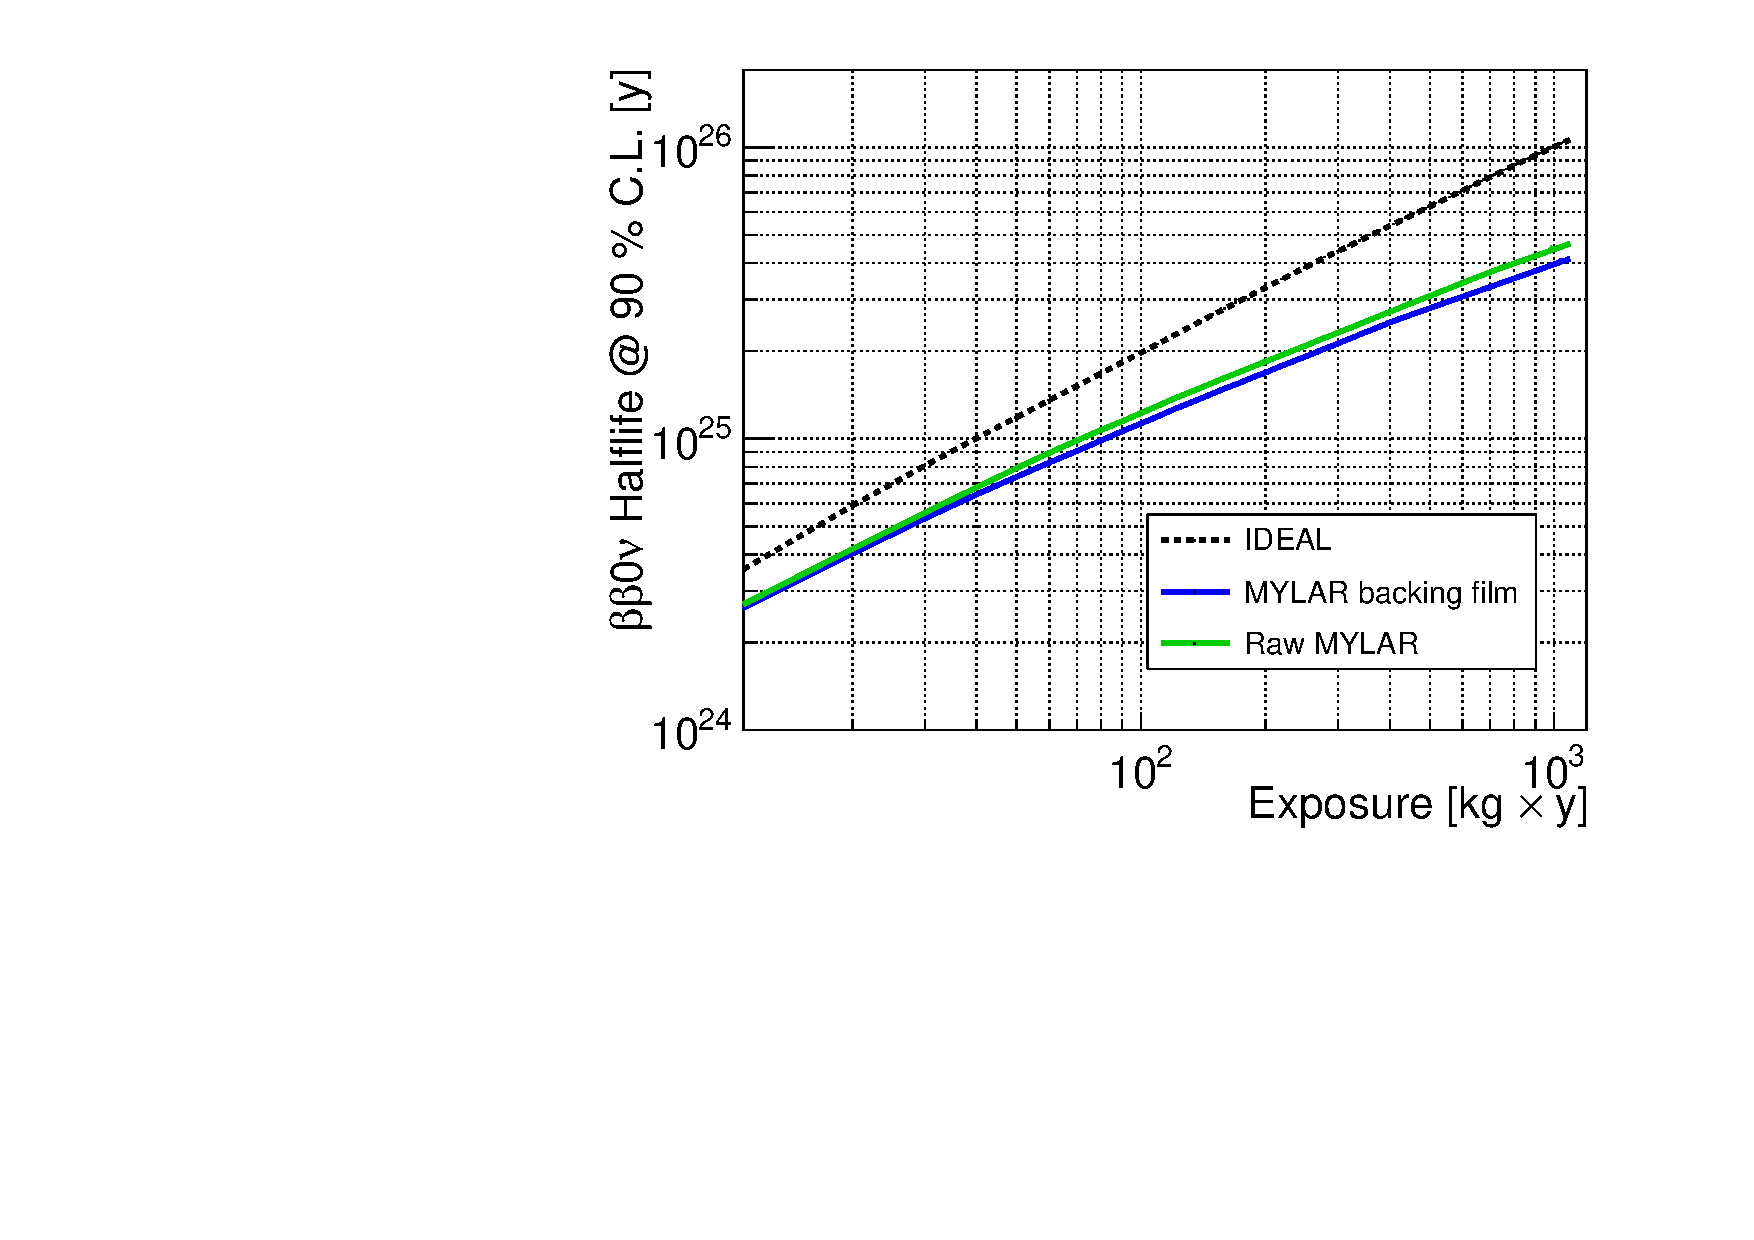
\includegraphics[scale=0.6]{pictures/Chap4/rawMylar.pdf}
\caption{SuperNEMO 0$\nu\beta\beta$ half-life limit at 90\% C.L. as a function of the exposure for the IDEAL, MYLAR backing film and raw MYLAR designs.}
\label{RawMylarDesignComparison}
\end{figure}

















\end{document}
